% CHAPTER 5: CORE AGENT IMPLEMENTATION
% ======================================================================
\section{Core Agent Implementation}

This chapter covers the three agent modules that form the platform's intelligence layer---tool agent, code agent, and RAG agent. Each section discusses internal architecture, key algorithms, and data flow design. Pseudocode tables and sequence diagrams are included to illustrate the operational logic of each agent.

\subsection{Tool Agent Implementation}

This agent runs within a separate tool-agent service (Spring Boot, port 8083), providing three capabilities: meeting room management, schedule conflict detection, and route planning. Technically, business logic is divided into REST endpoints and specialized service classes; the AI intent module provides a unified entry point for natural language input.

\subsubsection{Architecture and AI Intent Routing}

The tool agent employs a dual-path design at the interaction layer: one side retains programmatic calls, while the other open a natural language entry point.

Programmatic calls use a separate REST endpoint, where the frontend or third-party system directly passes type parameters, making the logic straightforward. Natural language interactions are uniformly sent to the /tool/execute endpoint. The DeepSeek LLM (Starfire API, accessed via the iFlytek MaaS platform) identifies the user's intent and extracts parameters from the natural language message. The request is then routed to the corresponding handler.

We separate the natural language entry point from the programmatic entry point, rather than using AI routing for everything, primarily for cost considerations. DeepSeek's token consumption and response latency are much higher than a direct REST call (roughly 500--800ms versus 5--10ms for a local call). In cases where the frontend already knows exactly what operation is to be performed (button clicks), calling the AI again would be both unnecessarily slow and a waste of tokens---adding extra cost for no benefit.

We ultimately adopted the iFlytek MaaS (Model as a Service) platform, which provide an interface compatible with the OpenAI Chat Completions format. Therefore, the underlying HTTP client can directly use the standard OpenAI library call pattern without modifying the request body structure.

\begin{figure}[H]
\centering
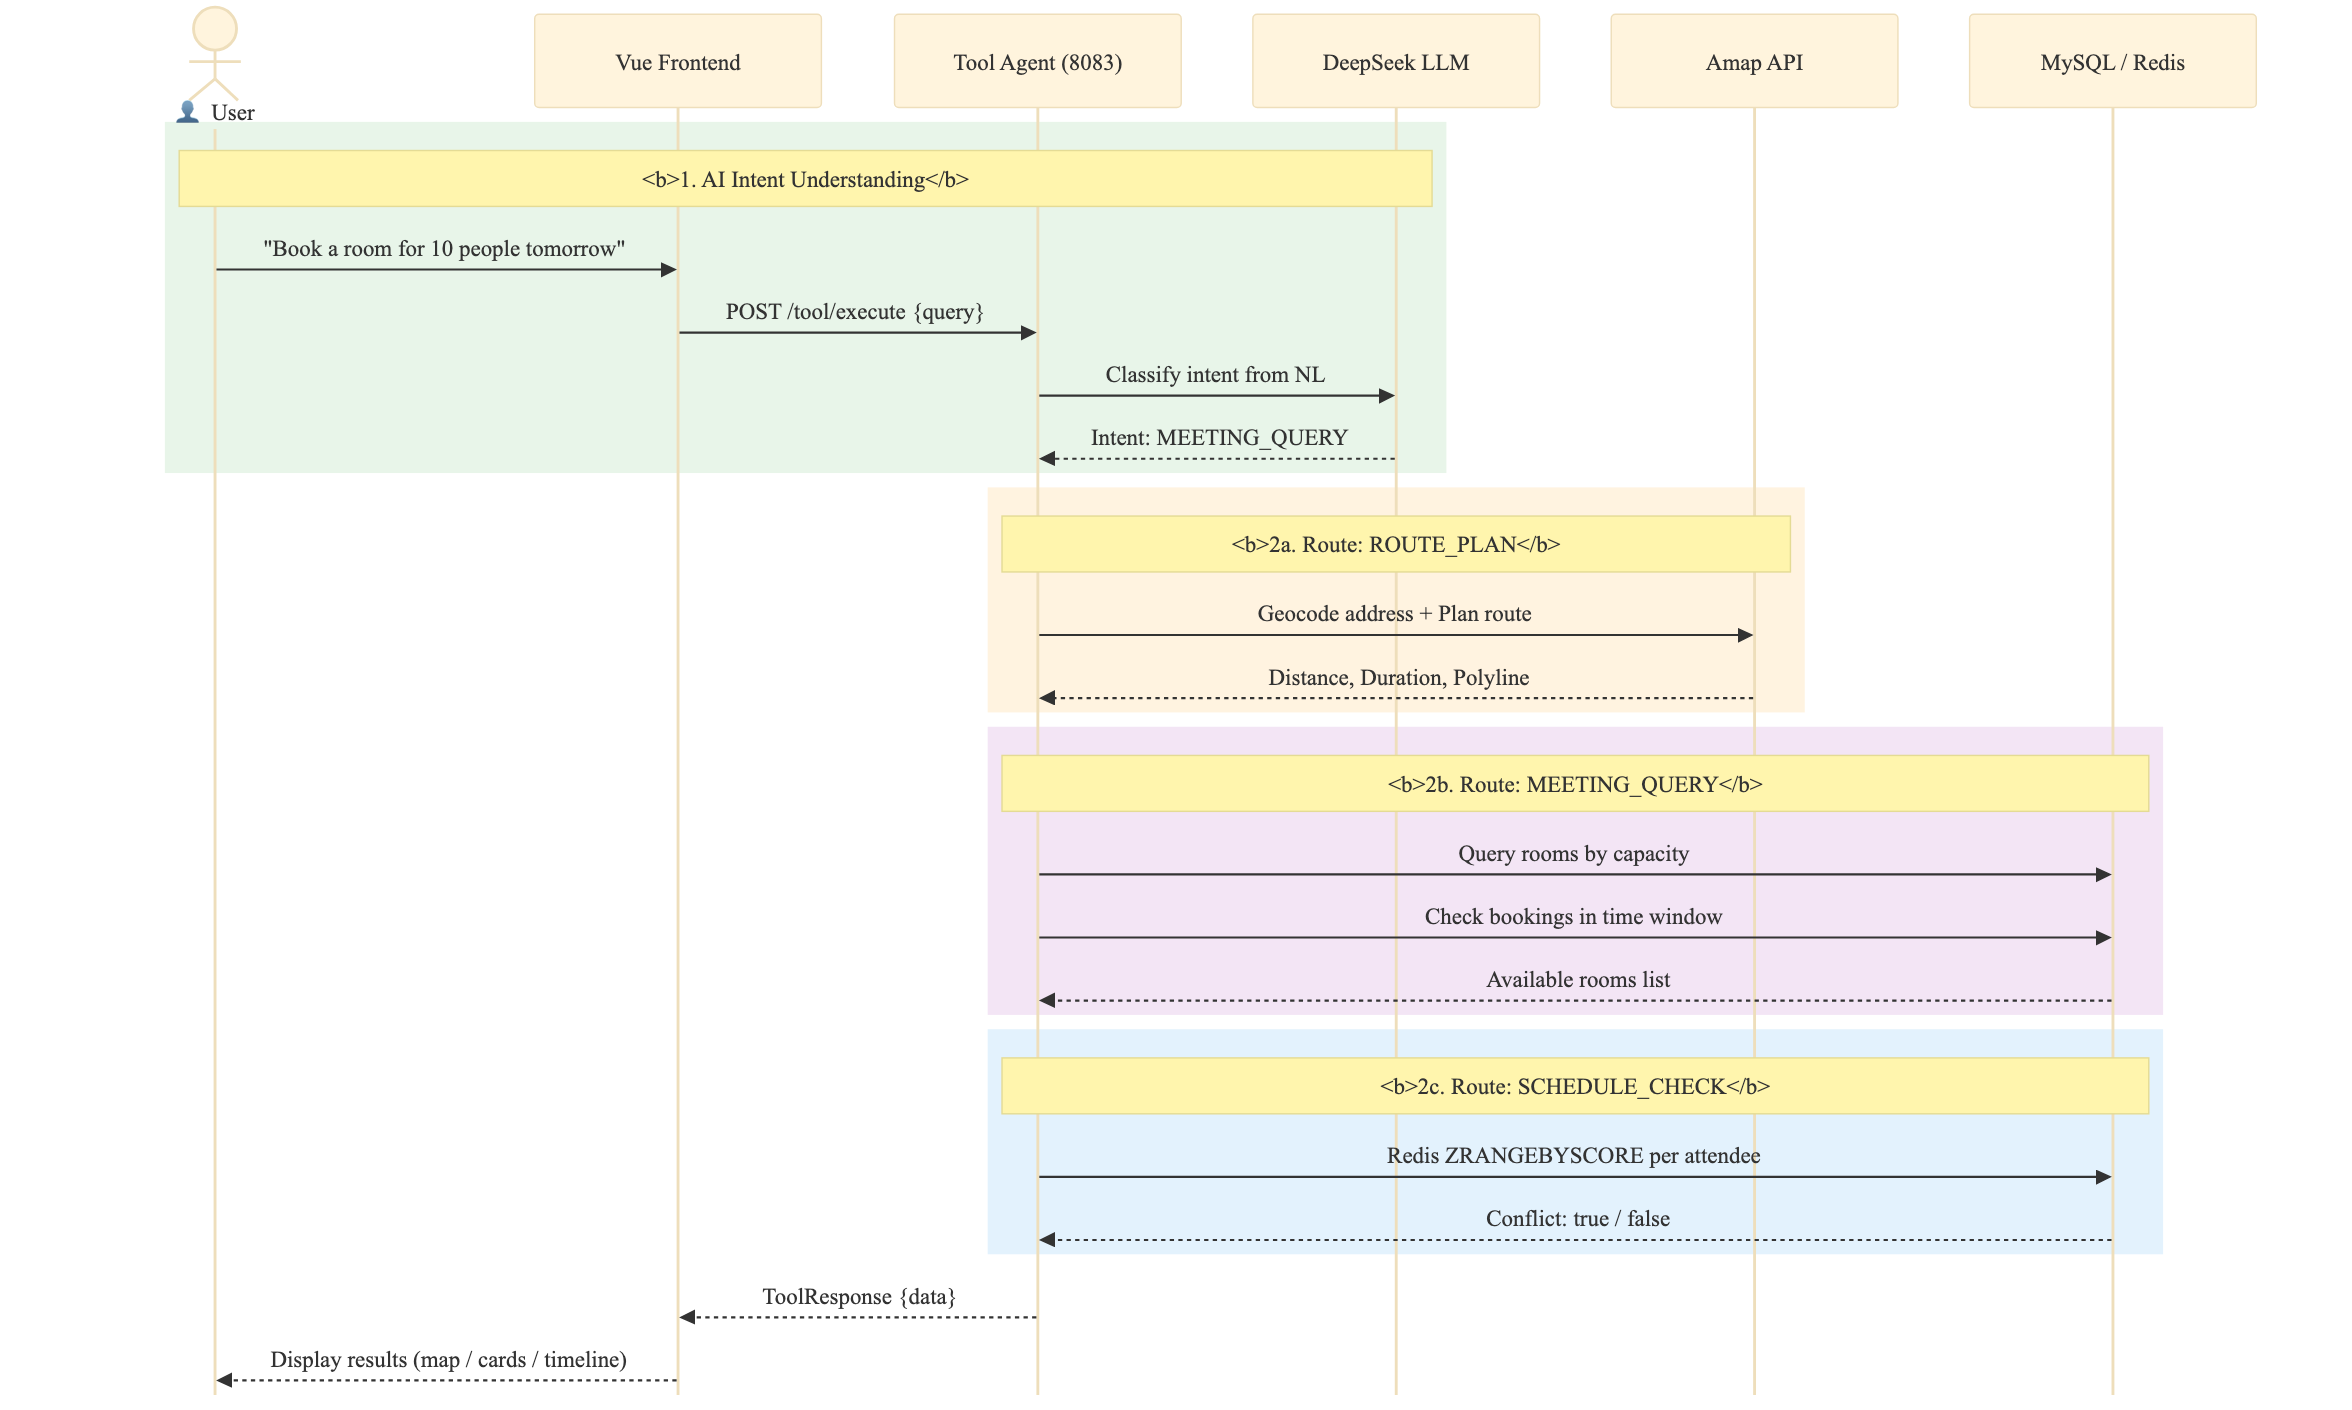
\includegraphics[width=0.92\textwidth]{figures/fig05_tool_agent_sequence.png}
\caption{Tool Agent Task Sequence --- DeepSeek AI Intent Routing to Specialized Handlers}
\label{fig:tool-agent-sequence}
\end{figure}

Tables \ref{tab:pseudocode-ai-intent} and \ref{tab:pseudocode-deepseek-chat} show the AI intent routing pipeline where DeepSeek classifies user input into three intent types and dispatches to the corresponding handler,  with a mock fallback on API failure.

\vspace{3mm}

\begin{table}[H]
\small\singlespacing
\centering
\caption{Pseudocode --- handleAiIntent() AI Intent Classification and Routing}
\label{tab:pseudocode-ai-intent}
\vspace{2mm}

\begin{lstlisting}
FUNCTION handleAiIntent(userInput: String): HandlerResult
    systemPrompt = PromptBuilder.create()
        .defineIntent("ROUTE_PLAN",
            params = ["from", "to", "mode"],
            description = "Route planning request")
        .defineIntent("MEETING_QUERY",
            params = ["date", "capacity", "equipment"],
            description = "Meeting room search")
        .defineIntent("SCHEDULE_CHECK",
            params = ["timeRange", "attendees"],
            description = "Schedule conflict detection")
        .build()
    response = deepSeekService.chat(
        system  = systemPrompt,
        user    = userInput,
        format  = "json_object",
        temp    = 0.3,
        maxTok  = 2048
    )
    intent = response.intentType
    params = response.parameters
    SWITCH intent:
        CASE "ROUTE_PLAN":
            RETURN routeHandler.handle(params.from, params.to, params.mode)
        CASE "MEETING_QUERY":
            RETURN meetingHandler.handle(params.date,
                       params.capacity, params.equipment)
        CASE "SCHEDULE_CHECK":
            RETURN scheduleHandler.handle(params.timeRange,
                       params.attendees)
        DEFAULT:
            THROW UnknownIntentException(intent)
    END SWITCH
END FUNCTION
\end{lstlisting}
\end{table}


\vspace{3mm}

\begin{table}[H]
\small\singlespacing
\centering
\caption{Pseudocode --- DeepSeekService.chat() LLM API Call with Fallback}
\label{tab:pseudocode-deepseek-chat}
\vspace{2mm}

\begin{lstlisting}
FUNCTION chat(system, user, format, temperature, maxTokens): DeepSeekResponse
    requestBody = {
        model:             config.deepseek.model,
        messages: [
            {role: "system", content: system},
            {role: "user",   content: user}
        ],
        response_format:   {type: format},
        temperature:       temperature,
        max_tokens:        maxTokens
    }
    TRY
        httpResponse = httpClient.send(
            method:  POST,
            url:     config.deepseek.baseUrl + "/chat/completions",
            headers: {
                "Authorization": "Bearer " + config.deepseek.apiKey,
                "Content-Type":  "application/json"
            },
            body:    toJSON(requestBody),
            timeout: 60s
        )
        rawJson = httpResponse.choices[0].message.content
        parsed  = objectMapper.readValue(rawJson, DeepSeekResponse)
        RETURN parsed   // {intentType, parameters}
    CATCH Exception e:
        log.error("DeepSeek API call failed", e)
        RETURN fallbackMock()   // demo data, source = "mock"
    END TRY
END FUNCTION
\end{lstlisting}
\end{table}


The DeepSeek API configuration in application.yml uses environment variables with development defaults: AI\_DEEPSEEK\_API\_KEY, AI\_DEEPSEEK\_BASE\_URL (defaulting to https://maas-api.cn-huabei-1.xf-yun.com/v1), AI\_DEEPSEEK\_MODEL (defaulting to deepseek-v3), AI\_DEEPSEEK\_TIMEOUT (180s), and AI\_DEEPSEEK\_MAX\_TOKENS (2000).

\subsubsection{Meeting Room Management}

For meeting room management, due to varying user permissions, we designed two sets of interfaces base on user permissions and functions:

The first set is for regular users. Regular users has a simple request: ``Check if there are any available rooms for this time slot.'' Therefore, our ToolController only includes a single GET request: /tool/meeting-rooms. Parameters include startTime, endTime, and capacity. The backend performs a three-phase availability check, as shown in the pseudocode in Table \ref{tab:pseudocode-query-rooms}.

The second set, the management side, uses a completely different logic (although the system administrator and department administrators maintain consistency). Because the Admin class needs to maintain meeting room resources, we provide a complete set of CRUD interfaces through MeetingRoomAdminController. In terms of security, it verifies the X-User-Roles header---this is simple but effective, because the header is injected by the gateway layer, not the client, and therefore cannot be forged.

\vspace{3mm}

\begin{table}[H]
\small\singlespacing
\centering
\caption{Pseudocode --- queryRoomsWithStatus() Three-Phase Room Availability Algorithm}
\label{tab:pseudocode-query-rooms}
\vspace{2mm}

\begin{lstlisting}
FUNCTION queryRoomsWithStatus(startTime, endTime, minCapacity): List<Map>
    // === Phase 1: Query all active meeting rooms ===
    query = new LambdaQueryWrapper<MeetingRoom>()
        .eq(MeetingRoom::status, 1)
    IF minCapacity <> NULL THEN
        query.ge(MeetingRoom::capacity, minCapacity)
    END IF
    rooms = meetingRoomMapper.selectList(query)

    // === Phase 2: Find booked room IDs in time range ===
    overlapping = bookingMapper.selectList(
        new LambdaQueryWrapper<MeetingSchedule>()
            .lt(MeetingSchedule::startTime, endTime)
            .gt(MeetingSchedule::endTime,   startTime)
    )
    bookedRoomIds = {b.roomId | b IN overlapping}

    // === Phase 3: Assemble availability response ===
    result = []
    FOR EACH room IN rooms:
        available = room.id NOT IN bookedRoomIds
        equipment = split(room.facilities, ",")
        result.add({
            id:          toString(room.id),
            name:        room.roomName,
            capacity:    room.capacity,
            location:    room.building + ", Floor " + room.floor,
            equipment:   equipment,
            available:   available,
            statusText:  IF available THEN "Available" ELSE "Booked",
            nextBooking: findNextBooking(room.id, startTime)
        })
    END FOR
    RETURN result
END FUNCTION
\end{lstlisting}
\end{table}


\vspace{3mm}

\begin{table}[H]
\small\singlespacing
\centering
\caption{Pseudocode --- bookRoom() Atomic Conflict Check-and-Insert}
\label{tab:pseudocode-book-room}
\vspace{2mm}

\begin{lstlisting}
FUNCTION bookRoom(roomId, startTime, endTime, booker, title): Long
    // Step 1 -- Atomic conflict check
    conflicts = scheduleMapper.selectCount(
        new LambdaQueryWrapper<MeetingSchedule>()
            .eq(MeetingSchedule::roomId,    roomId)
            .lt(MeetingSchedule::startTime, endTime)
            .gt(MeetingSchedule::endTime,   startTime)
    )
    IF conflicts > 0 THEN
        RETURN FALSE   // room already booked in this window
    END IF
    // Step 2 -- Insert new booking
    schedule = new MeetingSchedule()
    schedule.roomId    = roomId
    schedule.startTime = startTime
    schedule.endTime   = endTime
    schedule.booker    = booker
    schedule.title     = title
    schedule.status    = 1
    scheduleMapper.insert(schedule)
    RETURN schedule.id
END FUNCTION

FUNCTION getSchedulesForUsers(userIds, startTime, endTime): List<Schedule>
    RETURN scheduleMapper.selectList(
        new LambdaQueryWrapper<MeetingSchedule>()
            .in(MeetingSchedule::booker, userIds)
            .ge(MeetingSchedule::startTime, startTime)
            .le(MeetingSchedule::endTime,   endTime)
    )
END FUNCTION
\end{lstlisting}
\end{table}


The MeetingRoom entity (@TableName(``meeting\_room'')) maps to the database table with fields: id (Long, @TableId auto-increment), roomName (String), building (String, e.g., ``Building A''), floor (String, e.g., ``3F''), capacity (Integer), hasProjector/hasWhiteboard/hasVideoConf (Boolean), status (Integer, 0=available, 1=maintenance), and createTime (LocalDateTime).

Table \ref{tab:tool-agent-api} lists the Tool Agent REST API endpoints implemented in ToolController.

\vspace{3mm}

\begin{table}[H]
\small\singlespacing
\centering
\caption{Tool Agent REST API Endpoints}
\label{tab:tool-agent-api}
\vspace{2mm}

{\small\renewcommand{\arraystretch}{0.92}
\begin{tabular}{@{}p{1.5cm}p{3.5cm}p{4cm}p{\dimexpr\textwidth-9cm-6\tabcolsep\relax}@{}}
\toprule
\textbf{Method} & \textbf{Endpoint} & \textbf{Key Parameters} & \textbf{Description} \\
\midrule
POST   & /tool/execute          & toolType, naturalLanguage, parameters & Unified AI execution --- DeepSeek LLM classifies intent and routes to handler \\
GET    & /tool/meeting-rooms    & startTime, endTime, capacity         & Query rooms with time-based availability status and capacity filter \\
POST   & /tool/meeting-room/book & roomId, booker, startTime, endTime, topic & Atomic check-then-insert room booking with conflict verification \\
POST   & /tool/check-conflict   & attendees[], startTime, endTime      & Check schedule conflicts by attendee list via Redis ZRANGEBYSCORE \\
POST   & /tool/schedule/create  & userId, eventName, startTime, endTime & Create personal schedule (dual-write: MySQL room\_id=0 + Redis sorted set) \\
POST   & /tool/schedule/add     & userId, eventId, startTime, endTime  & Add schedule entry to Redis sorted set only \\
POST   & /tool/schedule/remove  & userId, eventId                      & Remove schedule entry from Redis sorted set by eventId prefix match \\
GET    & /tool/schedules        & date, users[]                        & Query schedules for specified users on a given date from MySQL \\
GET    & /tool/my-schedules     & X-User-Name header                   & Get authenticated user's bookings and personal schedules with room details \\
DELETE & /tool/my-schedule/\{id\} & X-User-Name header, path id          & Cancel schedule: set status=0 in MySQL, remove from Redis if personal \\
GET    & /tool/route            & from, to, mode (default driving)     & Plan route via Amap API with multi-level geocoding fallback and map data \\
\bottomrule
\end{tabular}
}
\end{table}


\subsubsection{Schedule Conflict Detection}

Schedule conflict detection uses a dual-layer architecture: MySQL is the persistent store for all schedule data, while Redis serves as a fast query cache for temporal overlap detection. The ScheduleService handles CRUD operations on meeting\_schedule records. Each schedule has a booker (the user who created it), optional room\_id (0 for personal schedules that don't need a room), start\_time/end\_time, and an attendees field stored as a comma-separated list. Each user's schedules are indexed in Redis as a sorted set, where scores represent epoch timestamps and members encode event identifiers plus time ranges---this structure allows O(log N) insertion and O(log N + M) range queries, where N is the number of schedules for that user and M is the number of results in the time window.

Figure \ref{fig:schedule-conflict} shows the schedule conflict detection algorithm.

\begin{figure}[H]
\centering
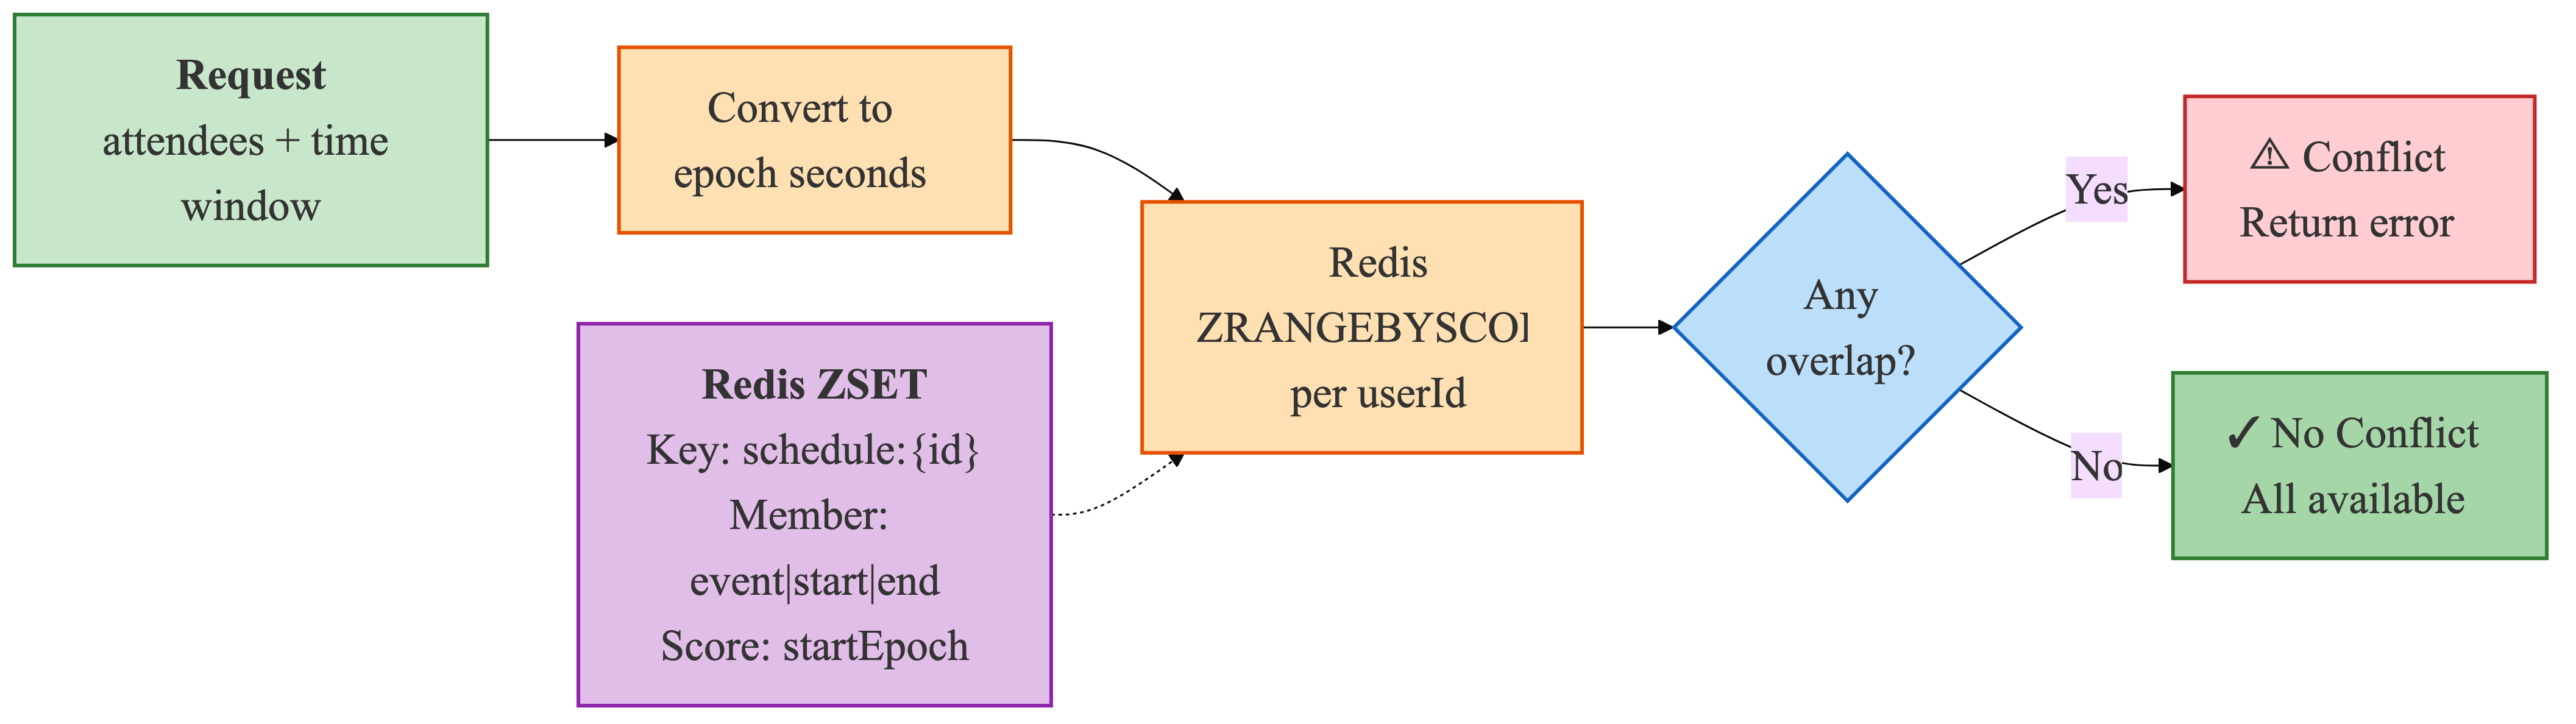
\includegraphics[width=0.92\textwidth]{figures/fig06_schedule_conflict.png}
\caption{Schedule Conflict Detection --- Redis Sorted Set-Based Temporal Overlap Algorithm}
\label{fig:schedule-conflict}
\end{figure}

Each user's schedules are stored in a Redis sorted set at key tool:schedule:\{userId\}. Schedule entries are encoded as members with the format ``\{eventId\}|\{startEpoch\}|\{endEpoch\}'', where startEpoch and endEpoch are Unix timestamps. For conflict detection queries, ZRANGEBYSCORE retrieves all schedule entries whose startEpoch is within the specified query window. For each retrieved schedule, the algorithm checks if the stored endEpoch overlaps with the query range to filter out partial overlaps.

Tables \ref{tab:pseudocode-redis-schedule}, \ref{tab:pseudocode-check-conflict}, and \ref{tab:pseudocode-dual-write} show the schedule management subsystem including Redis sorted-set operations for temporal conflict detection, attendee-based conflict checking,  and the MySQL-Redis dual-write consistency protocol.

\vspace{3mm}

\begin{table}[H]
\small\singlespacing
\centering
\caption{Pseudocode --- Redis Sorted Set Schedule Operations (add / remove / checkConflicts)}
\label{tab:pseudocode-redis-schedule}
\vspace{2mm}

\begin{lstlisting}
FUNCTION addSchedule(userId, eventId, startTime, endTime)
    key      = "tool:schedule:" + userId
    startTs  = toEpochMillis(startTime)
    endTs    = toEpochMillis(endTime)
    member   = eventId + ":" + startTs + ":" + endTs
    redisTemplate.opsForZSet().add(key, member, startTs)
END FUNCTION

FUNCTION removeSchedule(userId, eventId)
    key     = "tool:schedule:" + userId
    members = redisTemplate.opsForZSet().range(key, 0, -1)
    FOR EACH member IN members:
        IF member.startsWith(eventId + ":") THEN
            redisTemplate.opsForZSet().remove(key, member)
            BREAK
        END IF
    END FOR
END FUNCTION

FUNCTION checkConflicts(userId, startTime, endTime): List<String>
    key     = "tool:schedule:" + userId
    startTs = toEpochMillis(startTime)
    endTs   = toEpochMillis(endTime)
    // Query schedules whose start time falls within window
    overlapping = redisTemplate.opsForZSet()
        .rangeByScore(key, startTs, endTs)
    conflicts = []
    FOR EACH member IN overlapping:
        [evtId, memStartTs, memEndTs] = split(member, ":")
        IF parseLong(memStartTs) < endTs THEN
            conflicts.add(evtId)
        END IF
    END FOR
    RETURN conflicts
END FUNCTION
\end{lstlisting}
\end{table}


\vspace{3mm}

\begin{table}[H]
\small\singlespacing
\centering
\caption{Pseudocode --- POST /tool/check-conflict Attendee-Based Conflict Workflow}
\label{tab:pseudocode-check-conflict}
\vspace{2mm}

\begin{lstlisting}
ENDPOINT POST /tool/check-conflict
  Request:  {attendees: String[], startTime: String, endTime: String}
  Response: {hasConflict: Boolean, conflictUser: String?}

FUNCTION checkConflict(attendees, startTime, endTime): ConflictResult
    FOR EACH userId IN attendees:
        conflicts = scheduleService.checkConflicts(userId,
                        startTime, endTime)
        IF conflicts IS NOT EMPTY THEN
            // Early exit -- return first conflict found
            RETURN {
                hasConflict:  TRUE,
                conflictUser: userId,
                conflicts:    conflicts
            }
        END IF
    END FOR
    RETURN {hasConflict: FALSE, conflictUser: NULL}
END FUNCTION
\end{lstlisting}
\end{table}


\vspace{3mm}

\begin{table}[H]
\small\singlespacing
\centering
\caption{Pseudocode --- Schedule Dual-Write Pattern (MySQL + Redis Consistency)}
\label{tab:pseudocode-dual-write}
\vspace{2mm}

\begin{lstlisting}
// === Schedule Creation (dual-write) ===
ENDPOINT POST /tool/schedule/create
FUNCTION createSchedule(request): ScheduleResponse
    // Write 1 -- Persist to MySQL
    schedule = meetingRoomService.addPersonalSchedule({
        roomId:    0,       // personal schedule convention
        booker:    request.booker,
        startTime: request.startTime,
        endTime:   request.endTime,
        title:     request.title,
        status:    1
    })
    // Write 2 -- Cache to Redis for fast conflict queries
    eventId = "event_" + schedule.id
    scheduleService.addSchedule(request.booker, eventId,
                                 request.startTime, request.endTime)
    RETURN {scheduleId: schedule.id, eventId: eventId}
END FUNCTION

// === Schedule Cancellation (dual-delete) ===
ENDPOINT POST /tool/schedule/cancel
FUNCTION cancelSchedule(scheduleId): void
    // Step 1 -- Soft delete from MySQL (preserves audit trail)
    scheduleMapper.update(null,
        new LambdaUpdateWrapper<MeetingSchedule>()
            .eq(MeetingSchedule::id, scheduleId)
            .set(MeetingSchedule::status, 0)
            .set(MeetingSchedule::updateTime, now())
    )
    // Step 2 -- Remove from Redis cache
    scheduleService.removeSchedule(currentUser, "event_" + scheduleId)
END FUNCTION
\end{lstlisting}
\end{table}


\subsubsection{Route Planning}

The route planning feature integrates the Amap Open API through the AmapService class, which provides geocoding, route calculation, and map data for visualization. The GET /tool/route endpoint accepts origin, destination, and optional waypoint parameters, returning a route response containing path coordinates, turn-by-turn instructions, total distance, and estimated duration. geocoding (converting addresses to coordinates) is implemented through Amap's geocoding API, with detailed request parameters and LLM-based route description translation.

\begin{figure}[H]
\centering
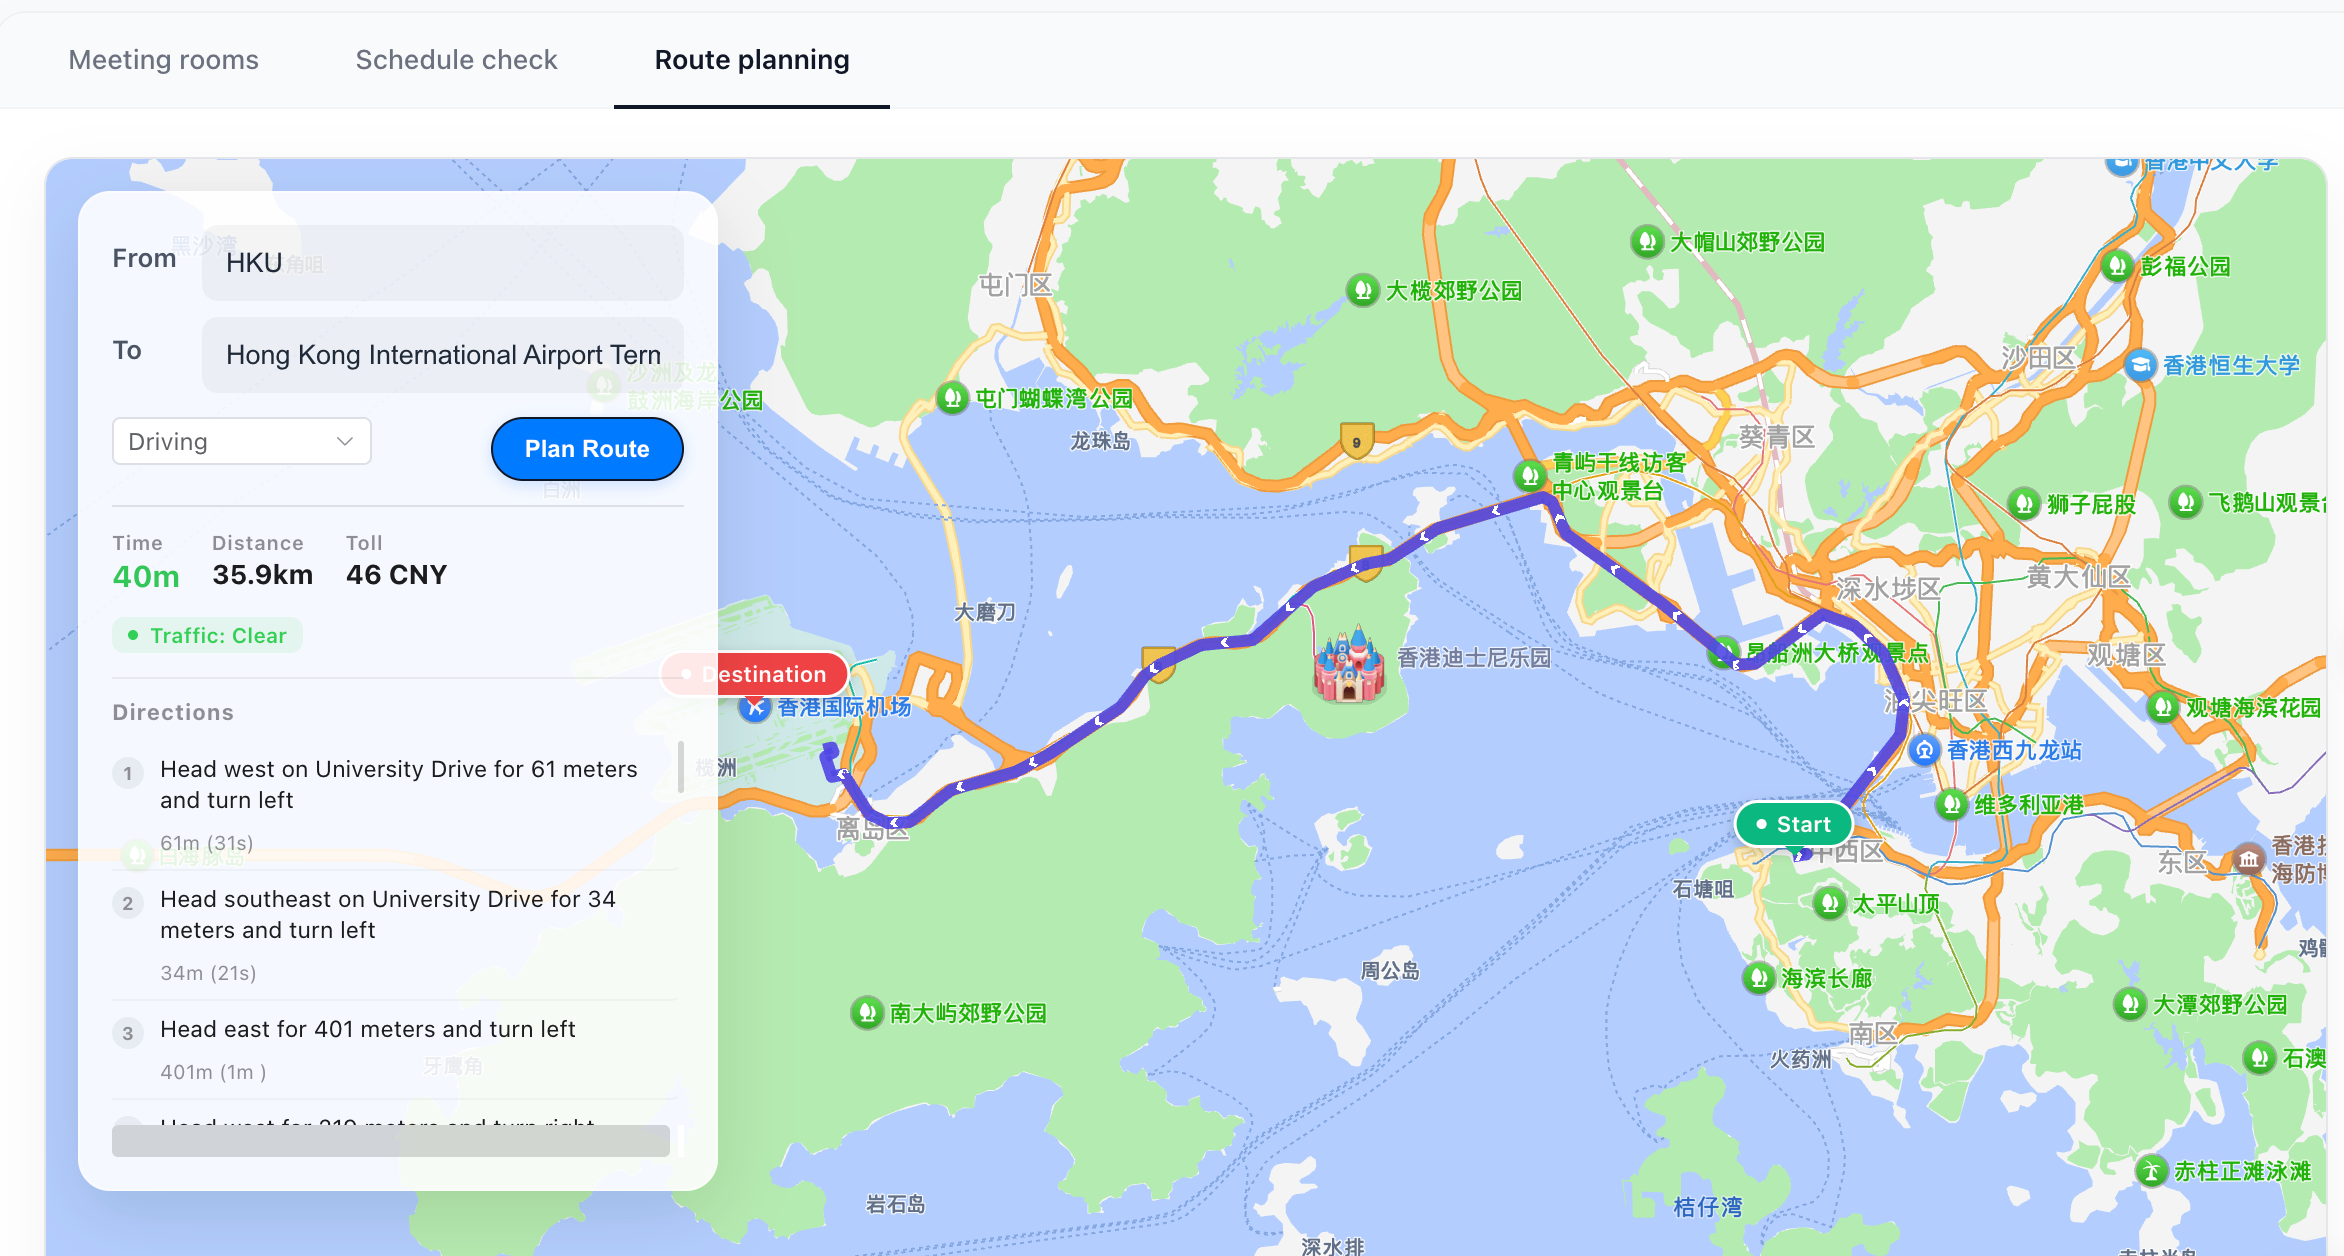
\includegraphics[width=0.92\textwidth]{figures/fig07_route_planning.png}
\caption{Route Planning Map Visualization --- Interactive Map with Route Polyline and Navigation Steps}
\label{fig:route-planning}
\end{figure}


\begin{table}[H]
\small\singlespacing
\centering
\caption{Route Planning Three-Stage Geocoding and Navigation Pipeline}
\label{tab:route-planning}
\vspace{2mm}

{\footnotesize\setlength{\tabcolsep}{3.5pt}
\begin{tabular}{@{}>{\raggedright\arraybackslash}p{1.4cm}>{\raggedright\arraybackslash}p{2.5cm}>{\raggedright\arraybackslash}p{3.5cm}>{\raggedright\arraybackslash}p{1.4cm}>{\raggedright\arraybackslash}p{2.0cm}>{\raggedright\arraybackslash}p{3.2cm}@{}}
\toprule
\textbf{Stage} & \textbf{Method} & \textbf{API Endpoint} & \textbf{Input} & \textbf{Output} & \textbf{Fallback} \\
\midrule
1 -- Geocoding  & geocode\-With\-Fallback() & \path{GET restapi.amap.com/v3/geocode/geo} & Address string & Location (lng,lat) & POI text search, prepend ``Beijing'' + retry \\
2 -- Route Calc & plan\-Driving\-Route()   & \path{GET restapi.amap.com/v3/direction/driving} & Origin + Dest coords, strategy (0--4) & Distance, duration, polyline steps & N/A --- returns error to caller \\
3 -- Enrichment & parse\-Route\-Result()   & --- (local processing) & Amap JSON response & Formatted text + coordinate arrays & N/A --- keeps raw values on parse error \\
\bottomrule
\end{tabular}
}
\end{table}


Table \ref{tab:pseudocode-geocode} shows the route geocoding pipeline with a three-level fallback strategy and LLM-based translation of navigation instructions.

\vspace{3mm}

\begin{table}[H]
\small\singlespacing
\centering
\caption{Pseudocode --- geocodeWithFallback() Multi-Level Address Resolution}
\label{tab:pseudocode-geocode}
\vspace{2mm}

\begin{lstlisting}
FUNCTION geocodeWithFallback(address: String): Location
    TRY
        response = httpGet(restapi.amap.com/v3/geocode/geo,
            {key: apiKey, address: URL_ENCODE(address)})
        IF response.geocodes IS NOT EMPTY THEN
            RETURN parseLocation(response.geocodes[0].location)
        END IF
    CATCH:  // fall through
    TRY
        // Fallback 1 -- POI text search
        response = httpGet(restapi.amap.com/v3/place/text,
            {key: apiKey, keywords: URL_ENCODE(address), offset: 1})
        IF response.pois IS NOT EMPTY THEN
            RETURN parseLocation(response.pois[0].location)
        END IF
    CATCH:  // fall through
    // Fallback 2 -- Prepend "Beijing" and retry geocoding
    RETURN geocodeWithFallback("Beijing " + address)
END FUNCTION

FUNCTION translateRouteToEnglish(routeData): RouteData
    fields = extractChineseFields(routeData)
    TRY
        translated = deepSeekService.chat(
            system = "Translate to English, keep JSON structure",
            user   = toJSON(fields),
            format = "json_object")
        RETURN replaceUnits(translated)
            // e.g., "km" instead of Chinese units
    CATCH:
        RETURN routeData   // keep original Chinese
    END TRY
END FUNCTION
\end{lstlisting}
\end{table}


On the frontend, the MapContainer.vue component loads the Amap JS API v2.0 SDK through script injection with the API key  and security code. The component creates a map instance with zoom level 12, centered on the starting coordinate. An indigo polyline renders the route path. Green and red custom marker icons indicate the start and end points, respectively. Turning instructions are displayed in a scrollable list below the map, with each instruction showing the road name, distance, and a directional icon.

\subsection{Code Agent Implementation}

The Code Agent lets users generate executable SQL queries from natural language descriptions, connecting business users' domain expertise with the SQL knowledge needed for direct database interaction.

\subsubsection{Architecture Overview}

Table \ref{tab:code-agent-pipeline} shows the four-stage pipeline of Code Agent.

\vspace{3mm}

\begin{table}[H]
\small\singlespacing
\centering
\caption{Code Agent Four-Stage Natural Language to SQL Pipeline}
\label{tab:code-agent-pipeline}
\vspace{2mm}

{\small
\begin{tabular}{@{}p{1.8cm}>{\raggedright\arraybackslash}p{3.8cm}p{4.3cm}>{\raggedright\arraybackslash}p{\dimexpr\textwidth-9.9cm-6\tabcolsep\relax}@{}}
\toprule
\textbf{Stage} & \textbf{Service Class} & \textbf{Key Operation} & \textbf{Security Mechanism} \\
\midrule
1 -- Metadata Extraction & Metadata\-Cache\-Service & Query information\_schema for table/column definitions; cache as JSON in Redis (key: code\_agent:metadata:tables) & Provides whitelists (table names, column names) to the validation layer \\
2 -- SQL Generation & Onnx\-Code\-Generation\-Service & HTTP POST \{question\} $\rightarrow$ Python LLM inference server (port 8090); receives \{sql, method\} & N/A --- generation only; output is untrusted at this stage \\
3 -- SQL Validation & Sql\-Validation\-Service & Five-layer defense-in-depth pipeline: (1) operation type, (2) forbidden keywords, (3) table whitelist, (4) column whitelist, (5) complexity limits & Blocks: non-SELECT, DDL/DML keywords, unrecognized tables/columns, overly complex queries \\
4 -- SQL Execution & Sql\-Execution\-Service & Re-validate (defense in depth) $\rightarrow$ execute via Jdbc\-Template with Prepared\-Statement & Parameterized queries prevent injection; read-only connection enforced \\
\bottomrule
\end{tabular}
}
\end{table}


The CodeAgentController exposes six endpoints: POST /code/query (one-shot generate and execute, returns FullResult with SQL, columns, rows, elapsedMs), POST /code/generate (preview only, generates SQL without execution), POST /code/execute (execute only, runs previously generated SQL), GET /code/metadata (returns cached schema metadata), POST /code/metadata/refresh (manually triggers schema refresh), and GET /code/health (returns service status and LLM connectivity).

Figure \ref{fig:code-agent-usecase} shows the Code Agent use case diagram. Business analysts interact with the system by submitting natural language queries through the three-step frontend interface. The system processes requests by encoding database schema information, sending structured prompts to the Python LLM inference server, receiving generated SQL, running it through the five-layer validation pipeline, executing only validated queries via JdbcTemplate against MySQL, and returning results with the generated SQL and execution metadata.

\begin{figure}[H]
\centering
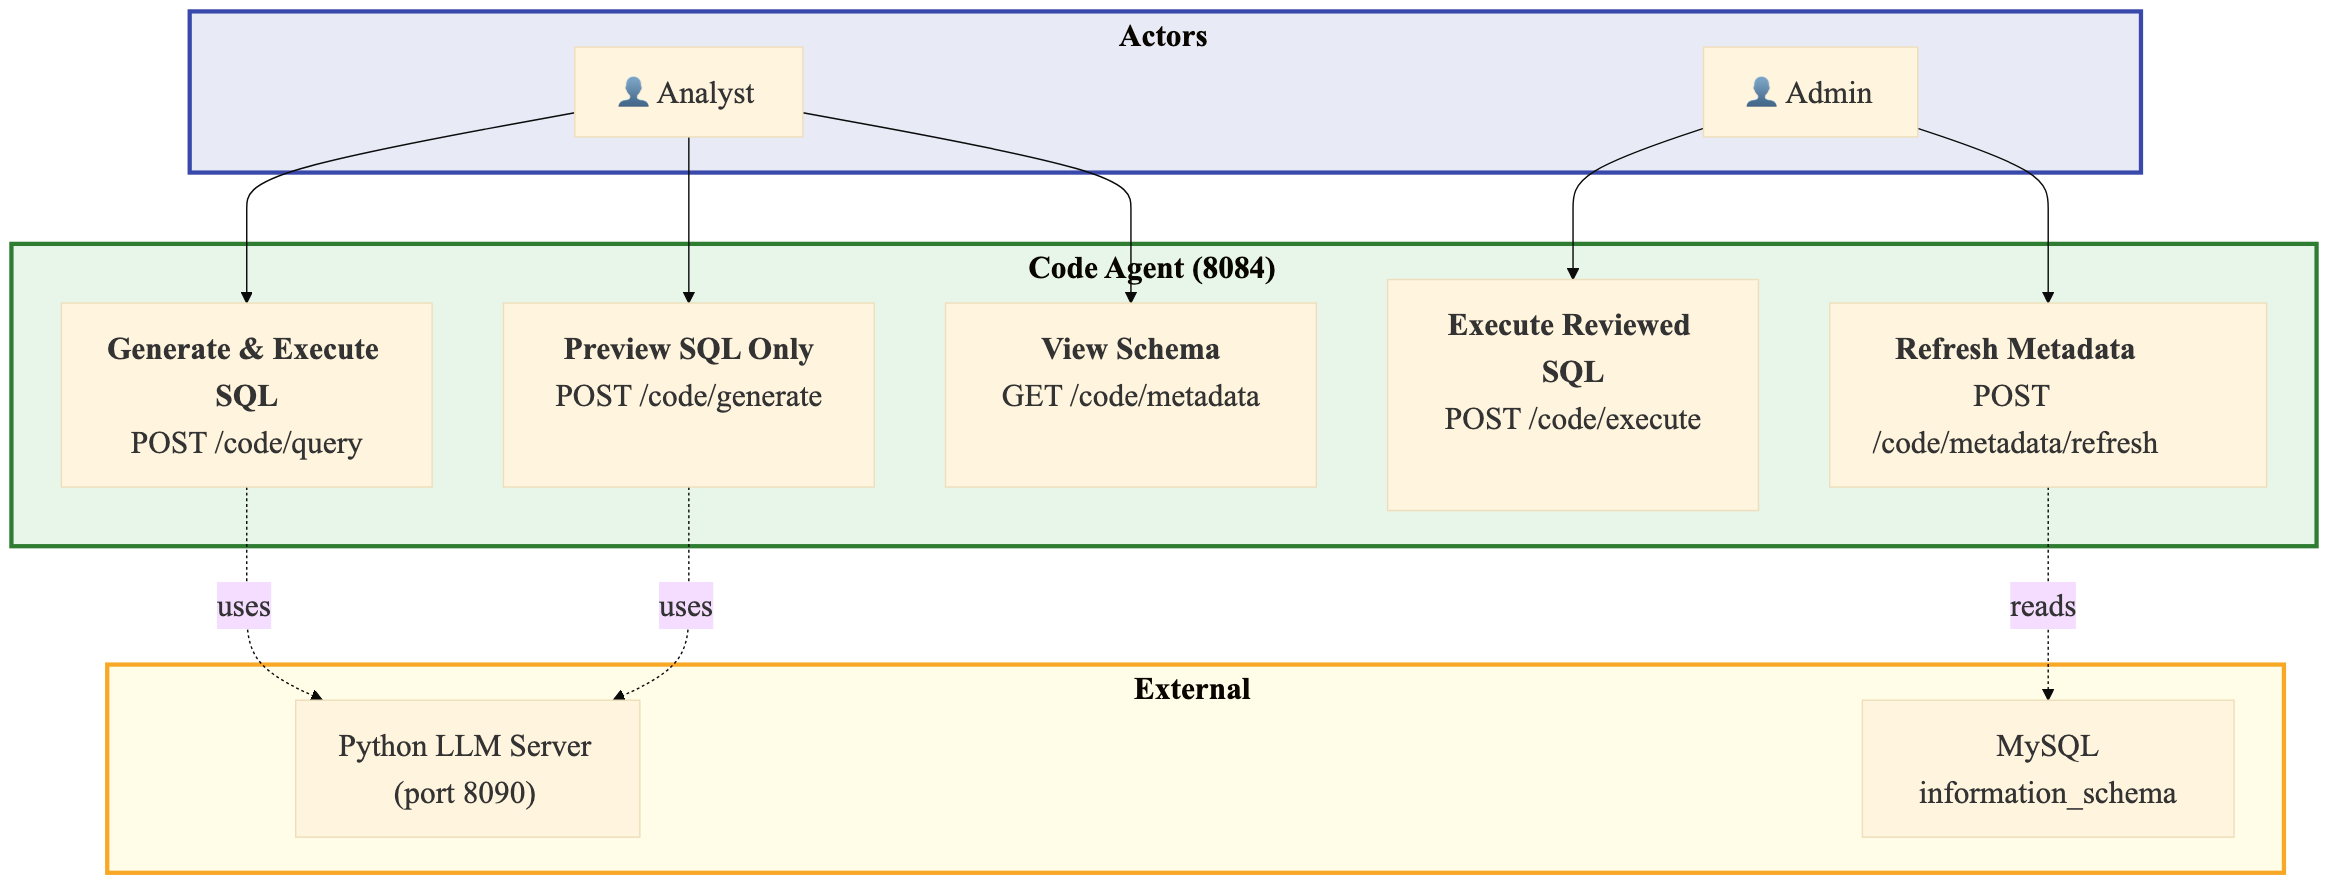
\includegraphics[width=0.92\textwidth]{figures/fig08_code_agent_usecase.png}
\caption{Code Agent Use Case Diagram --- Natural Language to Safe SQL Execution}
\label{fig:code-agent-usecase}
\end{figure}

The use case covers schema-aware query generation, five-layer security validation, JdbcTemplate-based execution, and result presentation with export capabilities.

\subsubsection{Python LLM Inference Server Integration}

Table \ref{tab:pseudocode-onnx} shows the SQL generation HTTP proxy that forwards natural language questions to the Python LLM inference server and parses the returned SQL.

\vspace{3mm}

\begin{table}[H]
\small\singlespacing
\centering
\caption{Pseudocode --- OnnxCodeGenerationService HTTP Proxy to Python Inference Server}
\label{tab:pseudocode-onnx}
\vspace{2mm}

\begin{lstlisting}
// @Service, @ConditionalOnProperty(code-agent.onnx.enabled=true)
// Acts as HTTP proxy (NOT direct ONNX Runtime inference)
FUNCTION generateSQL(question: String): CodeGenerationResponse
    payload = {question: question}
    TRY
        httpResponse = httpClient.send(
            method:  POST,
            url:     config.serverUrl,  // default: http://localhost:8090/infer
            headers: {"Content-Type": "application/json"},
            body:    toJSON(payload),
            connectTimeout: 10s,
            responseTimeout: 60s
        )
        responseBody = objectMapper.readTree(httpResponse.body)
        sql    = responseBody.get("sql").asText()
        method = responseBody.get("method").asText()
        IF sql IS BLANK THEN
            RETURN failure("Generated SQL is empty")
        END IF
        RETURN success(sql, method)
    CATCH Exception e:
        log.error("SQL generation failed", e)
        RETURN failure(e.message)
    END TRY
END FUNCTION

// Design note: Any LLM serving framework can back port 8090
// as long as it accepts {question} and returns {sql, method}.
// Reference: Python inference server at data/infer_server.py
// hosts fine-tuned T5 model (data/fine-tuned-t5-banking/).
\end{lstlisting}
\end{table}


\subsubsection{Five-Layer SQL Whitelist Validation}

The SqlValidationService uses a defense-in-depth validation pipeline with five sequential layers, each of which can reject SQL that violates its security rule. The validation is configurable through CodeAgentProperties in application.yml.

Figure \ref{fig:sql-validation} shows the pipeline from natural language input to safe SQL execution. The five validation layers run in sequence.

\begin{figure}[H]
\centering
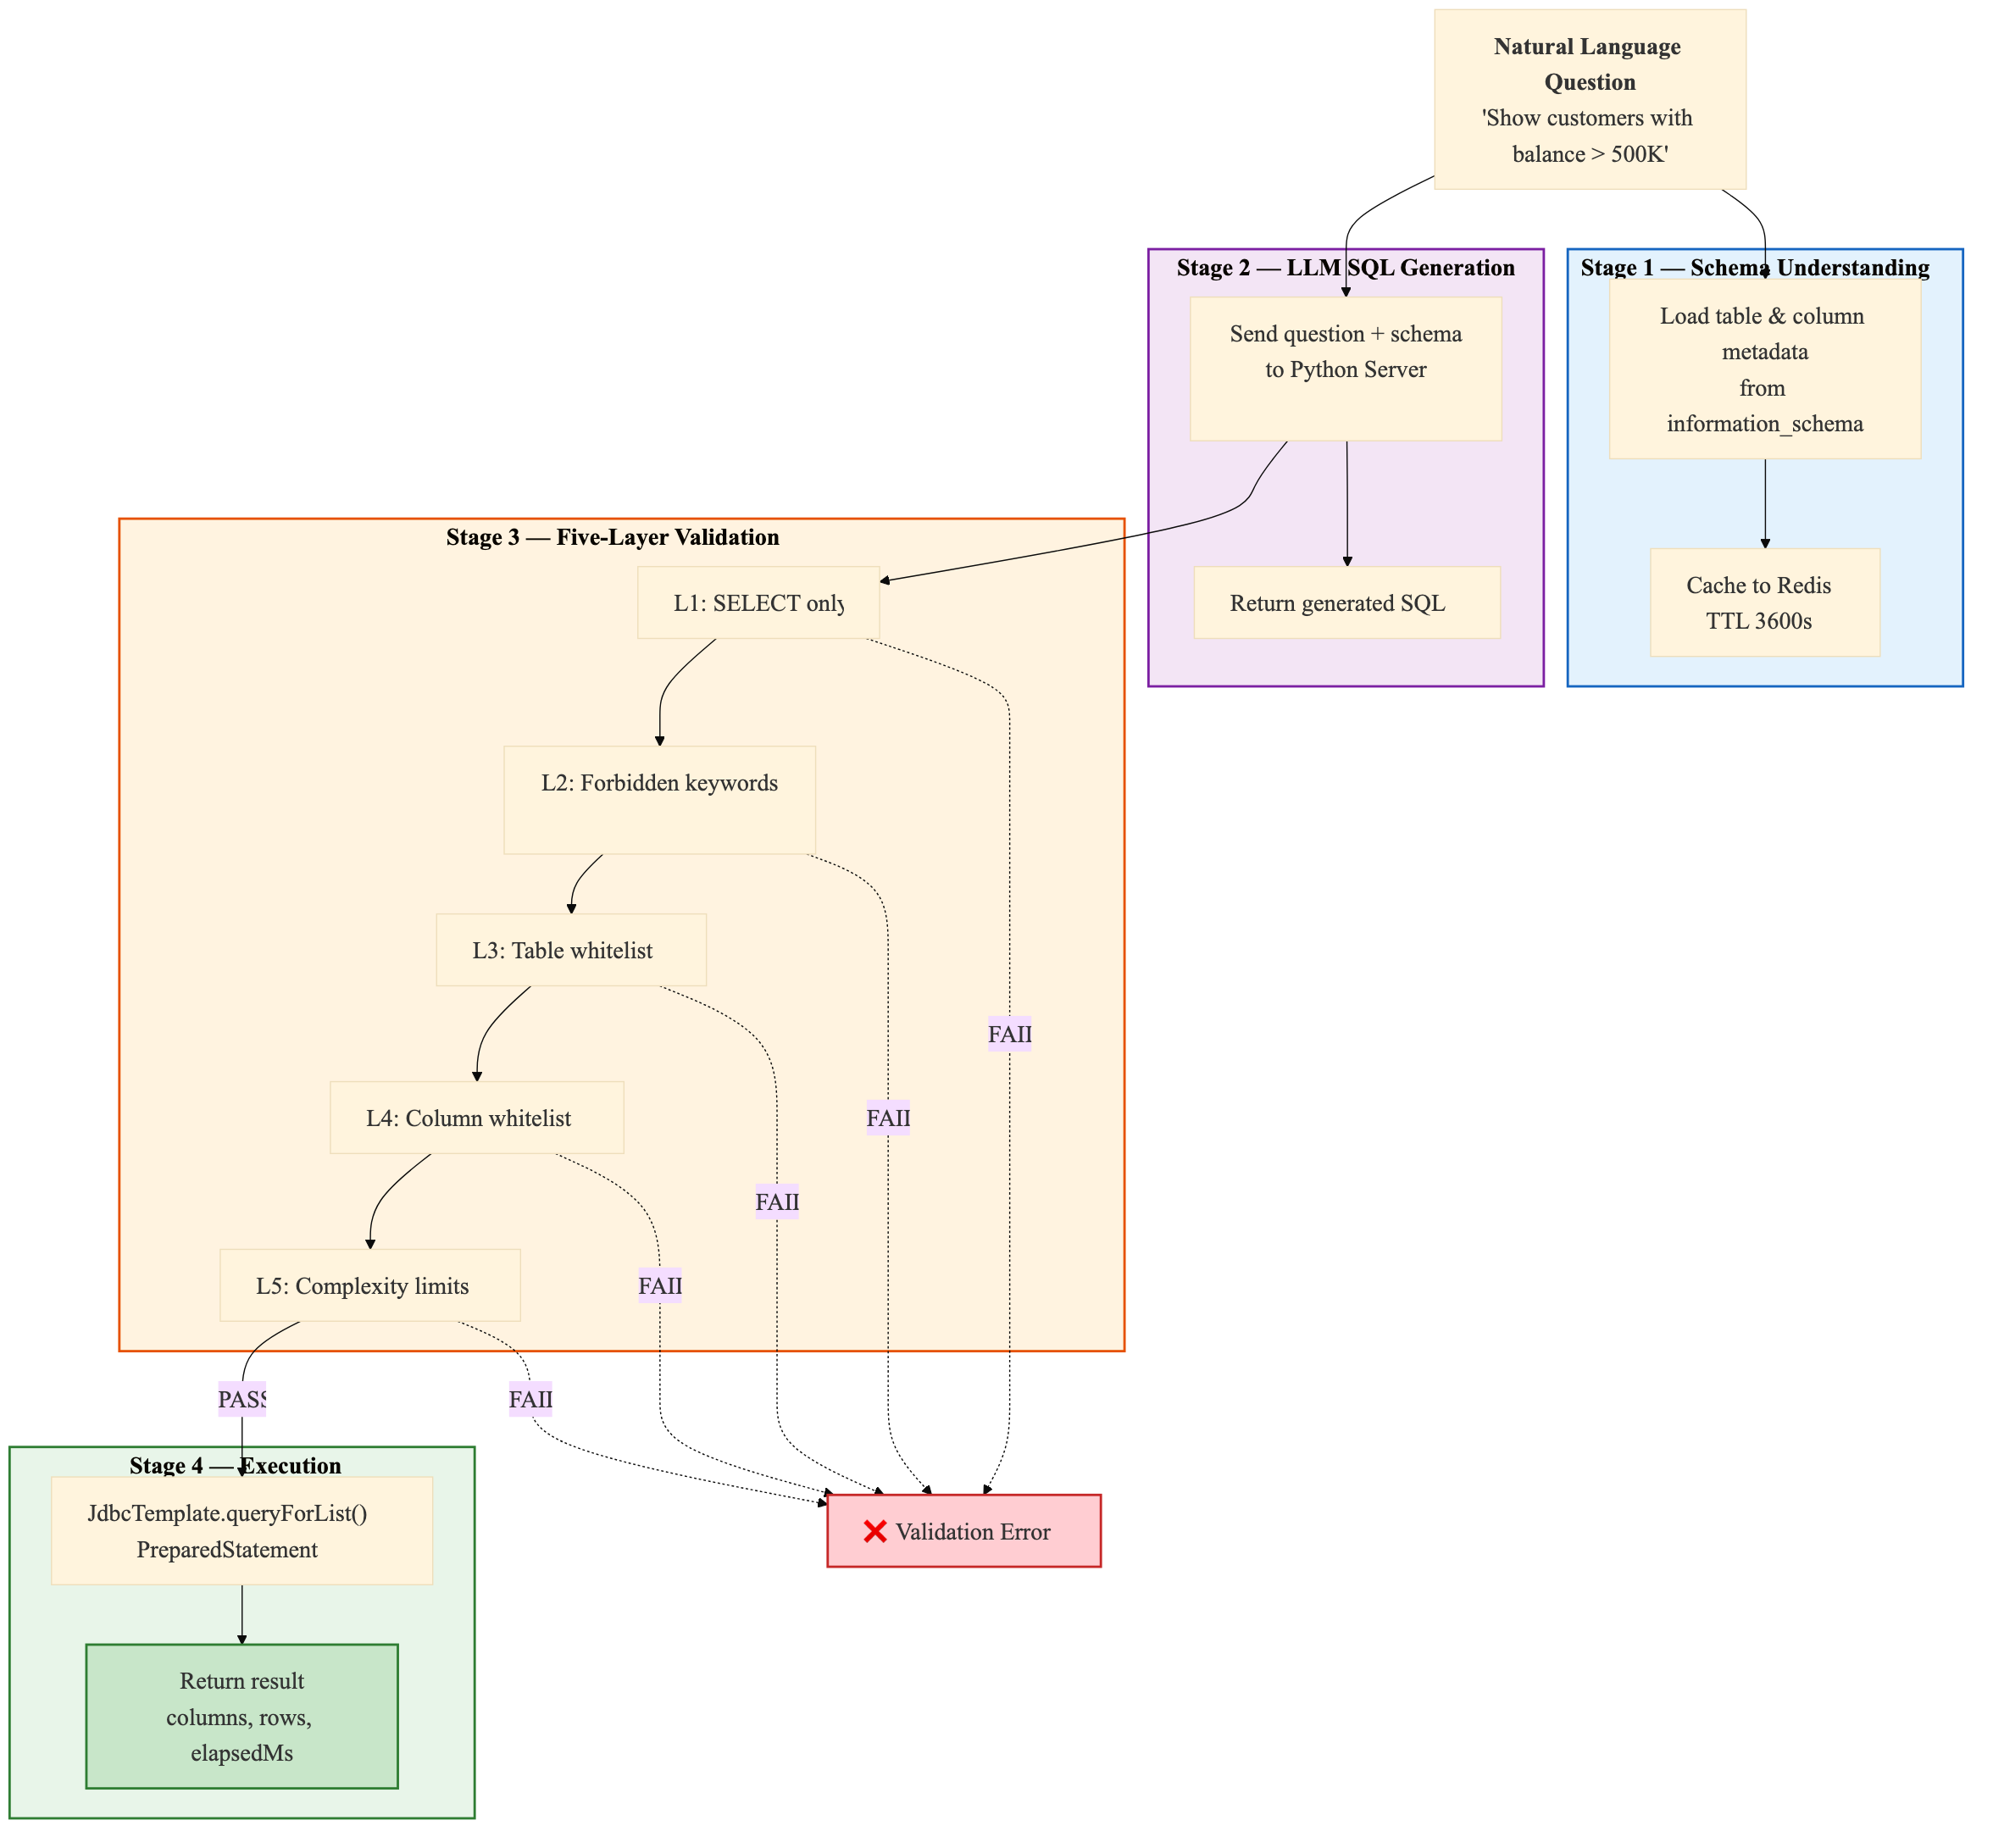
\includegraphics[width=0.92\textwidth]{figures/fig09_sql_validation.png}
\caption{SQL Generation and Five-Layer Validation Pipeline}
\label{fig:sql-validation}
\end{figure}

Tables \ref{tab:pseudocode-validate-op}, \ref{tab:pseudocode-validate-keywords}, \ref{tab:pseudocode-validate-tables}, \ref{tab:pseudocode-validate-cols}, and \ref{tab:pseudocode-validate-complexity} show the five-layer SQL whitelist validation pipeline: operation type restriction, forbidden keyword blacklist, table name whitelist, column  name whitelist, and query complexity limits.

\vspace{3mm}

\begin{table}[H]
\small\singlespacing
\centering
\caption{Pseudocode --- validateOperation() SQL Operation Type Check (Layer 1)}
\label{tab:pseudocode-validate-op}
\vspace{2mm}

\begin{lstlisting}
FUNCTION validateOperation(sql: String): ValidationResult
    normalized = collapseWhitespace(sql).trim().uppercase()
    allowedOps = config.getAllowedOperations()  // default: ["SELECT"]
    FOR EACH op IN allowedOps:
        IF normalized.startsWith(op) THEN
            RETURN PASS
        END IF
    END FOR
    RETURN FAIL("Only SELECT operations are permitted")
END FUNCTION
\end{lstlisting}
\end{table}


\vspace{3mm}

\begin{table}[H]
\small\singlespacing
\centering
\caption{Pseudocode --- validateForbiddenKeywords() Keyword Blacklist Scan (Layer 2)}
\label{tab:pseudocode-validate-keywords}
\vspace{2mm}

\begin{lstlisting}
FUNCTION validateForbiddenKeywords(sql: String): ValidationResult
    upperSQL = sql.uppercase()
    // Default blacklist: DROP, DELETE, INSERT, UPDATE, ALTER,
    //   TRUNCATE, CREATE, EXEC, EXECUTE, UNION, INTO,
    //   LOAD_FILE, OUTFILE, DUMPFILE
    FOR EACH keyword IN config.getForbiddenKeywords():
        pattern = "\\b" + keyword + "\\b"  // word-boundary regex
        IF pattern IS FOUND IN upperSQL THEN
            RETURN FAIL("Forbidden keyword detected: " + keyword)
        END IF
    END FOR
    RETURN PASS
END FUNCTION
\end{lstlisting}
\end{table}


\vspace{3mm}

\begin{table}[H]
\small\singlespacing
\centering
\caption{Pseudocode --- validateTableNames() Table Whitelist Verification (Layer 3)}
\label{tab:pseudocode-validate-tables}
\vspace{2mm}

\begin{lstlisting}
FUNCTION validateTableNames(sql: String): ValidationResult
    allowedTables = metadataCacheService.getAllowedTableNames()
    IF allowedTables IS EMPTY THEN
        log.warn("Metadata cache empty - skipping table whitelist")
        RETURN PASS   // skip when Redis/metadata unavailable
    END IF
    // Extract table references from FROM and JOIN clauses
    pattern = "\\b(?:FROM|JOIN)\\s+`?(\\w+)"  // case-insensitive
    extracted = findAllMatches(pattern, sql)
    FOR EACH tableName IN extracted:
        IF tableName NOT IN allowedTables THEN
            RETURN FAIL(
                "Table not allowed: " + tableName
                + ". Allowed: " + allowedTables)
        END IF
    END FOR
    RETURN PASS
END FUNCTION
\end{lstlisting}
\end{table}


\vspace{3mm}

\begin{table}[H]
\small\singlespacing
\centering
\caption{Pseudocode --- validateColumnNames() Column Whitelist Verification (Layer 4)}
\label{tab:pseudocode-validate-cols}
\vspace{2mm}

\begin{lstlisting}
FUNCTION validateColumnNames(sql: String): ValidationResult
    // Skip for SELECT * or SELECT COUNT(*) queries
    IF sql CONTAINS "SELECT *" OR sql CONTAINS "SELECT COUNT(*)" THEN
        RETURN PASS
    END IF
    allowedColumns = metadataCacheService.getAllowedColumns()
    IF allowedColumns IS EMPTY THEN
        log.warn("Metadata cache empty - skipping column whitelist")
        RETURN PASS   // skip when metadata unavailable
    END IF
    // Extract column spec between SELECT and FROM
    match = regex("SELECT\\s+(.+?)\\s+FROM", sql, CASE_INSENSITIVE)
    IF match NOT FOUND THEN
        RETURN PASS   // cannot parse, allow through
    END IF
    columnsPart = match.group(1)
    FOR EACH colSpec IN split(columnsPart, ","):
        colRef = extractColumnReference(colSpec)
        // Support both table.column and bare column
        IF colRef IS qualified (t.col) THEN
            IF colRef NOT IN allowedColumns[colRef.table] THEN
                RETURN FAIL("Column not allowed: " + colRef)
            END IF
        ELSE
            found = ANY table IN allowedColumns
                    WHERE colRef IN allowedColumns[table]
            IF NOT found THEN
                RETURN FAIL("Column not allowed: " + colRef)
            END IF
        END IF
    END FOR
    RETURN PASS
END FUNCTION
\end{lstlisting}
\end{table}


\vspace{3mm}

\begin{table}[H]
\small\singlespacing
\centering
\caption{Pseudocode --- validateComplexity() Query Complexity Limits (Layer 5)}
\label{tab:pseudocode-validate-complexity}
\vspace{2mm}

\begin{lstlisting}
FUNCTION validateComplexity(sql: String): ValidationResult
    // Count table references
    tableCount = countMatches(
        "\\b(?:FROM|JOIN)\\s+`?(\\w+)", sql)
    maxTables  = config.getMaxTablesPerQuery()  // default: 3
    IF tableCount > maxTables THEN
        RETURN FAIL(
            "Too many tables: " + tableCount
            + " (max: " + maxTables + ")")
    END IF
    // Count conditions (AND/OR + 1 for base condition)
    conditionCount = 1
        + countMatches("\\bAND\\b", sql)
        + countMatches("\\bOR\\b",  sql)
    maxConditions = config.getMaxConditions()  // default: 10
    IF conditionCount > maxConditions THEN
        RETURN FAIL(
            "Too many conditions: " + conditionCount
            + " (max: " + maxConditions + ")")
    END IF
    RETURN PASS
END FUNCTION
\end{lstlisting}
\end{table}


Table \ref{tab:sql-validation-rules} summarizes the five validation layers with their default configurations.

\vspace{3mm}

\begin{table}[H]
\small\singlespacing
\centering
\caption{SQL Whitelist Validation Rules (Five-Layer Defense)}
\label{tab:sql-validation-rules}
\vspace{2mm}

\begin{tabular}{@{}p{2cm}p{3.5cm}p{5cm}p{\dimexpr\textwidth-10.5cm-6\tabcolsep\relax}@{}}
\toprule
\textbf{Layer} & \textbf{Check} & \textbf{Default Configuration} & \textbf{Action on Violation} \\
\midrule
1. Operation    & SQL must start with allowed operation & [``SELECT''] only & Block execution, return error with permitted operations \\
2. Keywords     & Word-boundary regex blacklist scan & DROP, DELETE, INSERT, UPDATE, ALTER, TRUNCATE, CREATE, EXEC, EXECUTE, UNION, INTO, LOAD\_FILE, OUTFILE, DUMPFILE & Block execution, identify forbidden keyword \\
3. Table Names  & FROM/JOIN tables vs. information\_schema & All BASE TABLEs in agent\_platform database & Block execution, show allowed table set \\
4. Column Names & SELECT columns vs. table column definitions & Per referenced table from metadata cache; skip on empty cache & Block execution, identify invalid column \\
5. Complexity   & Table count + condition count & Max 3 tables, max 10 conditions (AND/OR count + 1) & Block execution, show actual vs.\ max counts \\
\bottomrule
\end{tabular}
\end{table}


\subsubsection{Metadata Caching and Execution}

Tables \ref{tab:pseudocode-refresh-metadata}, \ref{tab:pseudocode-cache-lifecycle}, and \ref{tab:pseudocode-sql-execution} show the schema metadata cache loading from information\_schema to Redis, the cache lifecycle management with scheduled refresh, and thedefense-in-depth SQL execution flow.

\vspace{3mm}

\begin{table}[H]
\small\singlespacing
\centering
\caption{Pseudocode --- refreshAllMetadata() Schema Metadata Cache Loading}
\label{tab:pseudocode-refresh-metadata}
\vspace{2mm}

\begin{lstlisting}
FUNCTION refreshAllMetadata(): Map<String, TableMetadata>
    conn = dataSource.getConnection()
    database = config.getDatabaseName()
    // Query 1 -- All BASE TABLE names
    tables = conn.query(
        "SELECT TABLE_NAME FROM information_schema.TABLES
         WHERE TABLE_SCHEMA = ? AND TABLE_TYPE = 'BASE TABLE'",
        database)
    metadataMap = {}
    FOR EACH tableName IN tables:
        // Query 2 -- Column metadata
        columns = conn.query(
            "SELECT COLUMN_NAME, DATA_TYPE, IS_NULLABLE,
                    COLUMN_COMMENT, COLUMN_KEY
             FROM information_schema.COLUMNS
             WHERE TABLE_SCHEMA = ? AND TABLE_NAME = ?
             ORDER BY ORDINAL_POSITION",
            database, tableName)
        // Query 3 -- Table comment
        comment = conn.querySingle(
            "SELECT TABLE_COMMENT FROM information_schema.TABLES
             WHERE TABLE_SCHEMA = ? AND TABLE_NAME = ?",
            database, tableName)
        metadataMap[tableName] = {
            columns: columns,
            comment: comment
        }
    END FOR
    conn.close()
    // Serialize and cache to Redis
    json = objectMapper.writeValueAsString(metadataMap)
    redisTemplate.opsForHash().put(
        "code_agent:metadata", "tables", json)
    redisTemplate.expire(
        "code_agent:metadata", config.getCacheTtl())  // default: 3600s
    RETURN metadataMap
END FUNCTION
\end{lstlisting}
\end{table}


\vspace{3mm}

\begin{table}[H]
\small\singlespacing
\centering
\caption{Pseudocode --- MetadataCacheManager Cache Lifecycle Management}
\label{tab:pseudocode-cache-lifecycle}
\vspace{2mm}

\begin{lstlisting}
// @Component - manages metadata cache lifecycle

// === Startup - initial cache load ===
@EventListener(ApplicationReadyEvent)
FUNCTION onApplicationReady():
    TRY
        metadataCacheService.refreshAllMetadata()
        log.info("Metadata cache loaded successfully")
    CATCH Exception e:
        log.warn("Database not ready. Manually refresh via:")
        log.warn("  POST /api/code/metadata/refresh")
    END TRY
END FUNCTION

// === Periodic refresh - every 30 minutes ===
@Scheduled(fixedRate = 1800000)
FUNCTION scheduledRefresh():
    TRY
        metadataCacheService.refreshAllMetadata()
    CATCH Exception e:
        log.error("Scheduled metadata refresh failed", e)
    END TRY
END FUNCTION

// === Fallback - direct query when Redis unavailable ===
FUNCTION getAllTableMetadata(): Map<String, TableMetadata>
    TRY
        cached = redisTemplate.opsForHash()
            .get("code_agent:metadata", "tables")
        IF cached NOT NULL THEN
            RETURN deserializeJSON(cached)
        END IF
    CATCH:  // Redis unavailable - fall through
    // Direct DB query as fallback
    RETURN refreshAllMetadata()
END FUNCTION
\end{lstlisting}
\end{table}


\vspace{3mm}

\begin{table}[H]
\small\singlespacing
\centering
\caption{Pseudocode --- SqlExecutionService Defense-in-Depth SQL Execution}
\label{tab:pseudocode-sql-execution}
\vspace{2mm}

\begin{lstlisting}
FUNCTION execute(sql: String): QueryResult
    // Defense in depth - re-validate even from trusted pipeline
    validation = sqlValidationService.validate(sql)
    IF validation IS NOT PASS THEN
        RETURN failure(validation.errorMessage)
    END IF
    // Execute via PreparedStatement (JdbcTemplate handles this)
    TRY
        rows = jdbcTemplate.queryForList(sql)
        RETURN success({
            columns:   extractColumnNames(rows),
            data:      rows,
            rowCount:  rows.size(),
            elapsedMs: measureElapsed()
        })
    CATCH DataAccessException e:
        RETURN failure("Query execution failed: " + e.message)
    END TRY
END FUNCTION

FUNCTION generateAndExecute(question, generationService): FullResult
    genResult = generationService.generateSQL(question)
    IF genResult IS FAILURE THEN
        RETURN FullResult.failure(genResult.error)
    END IF
    execResult = execute(genResult.sql)
    RETURN FullResult({
        success:         execResult.success,
        sql:             genResult.sql,
        inferenceMethod: genResult.method,
        columns:         execResult.columns,
        rows:            execResult.data,
        rowCount:        execResult.rowCount,
        elapsedMs:       execResult.elapsedMs
    })
END FUNCTION
\end{lstlisting}
\end{table}


\subsection{RAG Agent Implementation}

\subsubsection{Design Rationale}

The RAG Agent is designed as the knowledge layer of the multi-agent banking platform rather than as a standalone document chatbot. Its responsibility is to transform heterogeneous enterprise documents into reusable, searchable, citable, and governable knowledge that can support both direct user questions and downstream agent workflows. In a simple RAG demonstration, the main objective is usually to retrieve semantically similar passages and place them in the prompt. In this system, retrieval is only one part of a broader \textbf{knowledge-to-answer lifecycle}: documents must be ingested, chunked, embedded, indexed, selected as evidence, synthesized into grounded answers, exposed through stable APIs, and recorded for later inspection.

This broader lifecycle requires the RAG Agent to balance four requirements at the same time. First, answers must be semantically relevant to the user's question. Second, every answer should be grounded in identifiable document chunks so that the source can be inspected. Third, the vector index must remain reproducible across embedding profiles and document updates. Fourth, enterprise access rules must be preserved before knowledge is passed to the language model. Therefore, the design treats RAG as a \textbf{governed evidence selection and synthesis} problem rather than a simple vector-search problem.

Formally, for a user $u$ and question $q$, the system first computes the accessible document set $A(u)$ from role, department, clearance level, and temporary approvals. Let $C(q)$ denote the candidate chunk set and $\mathrm{doc}(c)$ denote the source document of chunk $c$. The final evidence set is selected as:

\[
E_k(q,u)=\mathrm{TopK}_{\mathrm{sim}(e(q),e(c))}
\{c \in C(q) \mid \mathrm{doc}(c)\in A(u)\}
\]

This formulation is used together with document lifecycle management and grounded generation. Indexing records provenance before query time; retrieval selects semantically useful chunks under the active embedding profile and access context; generation synthesizes only the selected evidence; and query logs store enough metadata to reconstruct which documents were retrieved, excluded, cited, and used. The result is a RAG service whose output is not only an answer, but also an inspectable evidence package.

Table \ref{tab:rag-design-rationale} summarizes the design difference between ordinary RAG and the enterprise RAG model implemented in this project.

\vspace{3mm}

\begin{table}[H]
\small\singlespacing
\centering
\caption{Ordinary RAG vs. Enterprise RAG Design Requirements}
\label{tab:rag-design-rationale}
\vspace{2mm}

\begin{tabularx}{\textwidth}{>{\RaggedRight\arraybackslash}p{0.23\textwidth}>{\RaggedRight\arraybackslash}p{0.33\textwidth}>{\RaggedRight\arraybackslash}X}
\toprule
\textbf{Dimension} & \textbf{Ordinary RAG} & \textbf{Enterprise RAG in This System} \\
\midrule
Knowledge lifecycle & Documents are often preprocessed manually before the demo & Upload, parsing, chunking, vector upsert, rebuild, deletion, and readiness checks are managed as service operations \\
Retrieval objective & Return the most semantically similar chunks & Select evidence by combining semantic relevance, source provenance, embedding profile, and access context \\
Answer grounding & Context is mainly a prompt construction detail & Evidence is a first-class object with citations, chunk IDs, document IDs, scores, and snippets \\
Platform integration & Usually implemented as a page-level chatbot & Exposed as reusable APIs for the RAG workbench, Task Center, Copilot dispatch, and asynchronous task history \\
Model operation & One embedding space and one vector collection are usually assumed & Embedding profiles isolate BGE-M3 and Qwen vectors into separate collections with rebuild-required status tracking \\
Governance and observability & Logs often contain only question and answer text & Query logs, traceId, blocked counts, latency, profile metadata, and citation records make behavior inspectable \\
\bottomrule
\end{tabularx}
\end{table}

\subsubsection{Architecture Overview}

The RAG Agent is implemented as an independent Spring Boot microservice on port 8085. Its role is not merely to wrap Milvus or expose a document-search endpoint. Instead, it coordinates the complete knowledge-to-answer lifecycle: document ingestion, structure-aware chunking, embedding, vector indexing, evidence retrieval, grounded answer generation, citation construction, permission evaluation, and query audit logging. The service is exposed through Spring Cloud Gateway under /api/rag/**. Gateway authentication remains the entry point for user context: JwtAuthGlobalFilter validates the JWT token and forwards X-User-Id, X-User-Name, X-User-Dept-Id, X-User-Roles, and X-User-Security-Level headers to rag-agent.

Table \ref{tab:rag-agent-pipeline} summarizes the internal pipeline. Compared with the Code Agent, which mainly converts natural-language requests into validated database operations, the RAG Agent converts unstructured enterprise documents into grounded answers that can be inspected, reused, and orchestrated by other platform modules. The main technical challenge is therefore not only finding similar text, but preserving document structure, embedding-profile consistency, evidence quality, access context, citation traceability, and runtime observability throughout the pipeline.

\vspace{3mm}

\begin{table}[H]
\small\singlespacing
\centering
\caption{RAG Agent End-to-End Pipeline}
\label{tab:rag-agent-pipeline}
\vspace{2mm}

{\small
\begin{tabular}{@{}p{1.8cm}>{\raggedright\arraybackslash}p{3.3cm}p{4.3cm}>{\raggedright\arraybackslash}p{\dimexpr\textwidth-9.4cm-6\tabcolsep\relax}@{}}
\toprule
\textbf{Stage} & \textbf{Service / Component} & \textbf{Key Operation} & \textbf{Persisted State / Platform Result} \\
\midrule
1 -- Request Admission & Gateway + RagController & Authenticate JWT; forward user identity, department, role, and clearance headers & Reject unauthenticated requests before they reach retrieval logic \\
2 -- Access Context & RagPermissionService & Compute accessible document IDs from department scope, clearance level, admin role, temporary RAG\_APPLY approvals, and approval expiry & Produces the access context used for scoped vector search and post-retrieval verification \\
3 -- Query Embedding & EmbeddingClient & Encode the user question with the active embedding profile & Records embedding profile, model, dimension, and collection for audit \\
4 -- Vector Retrieval & VectorStoreService / \newline REST Milvus adapter & ANN search with COSINE similarity, a 4x over-fetch candidate size, and an allowed-document filter in Milvus & Produces ranked candidate chunks under the active profile and access context \\
5 -- Evidence Selection & RagQueryService & Re-rank and re-check candidate chunks; build the final evidence set before prompt construction & Records retrieved document IDs, excluded document IDs, and selected chunks \\
6 -- Grounded Generation & Query prompt logic + \newline RagLlmClient & Build evidence-only prompt; call OpenAI-compatible chat-completions endpoint & Produces answer text and citation references from selected evidence chunks \\
7 -- Response + Audit & Query service + \newline query log mapper & Return traceId, answer, citations, scores, and latency; persist query log & Enables later review of evidence, blocked docs, profile, and timing \\
\bottomrule
\end{tabular}
}
\end{table}

Figure \ref{fig:rag-agent-architecture} shows the two parallel flows inside the RAG Agent: the indexing flow that prepares document vectors, and the query flow that retrieves evidence and generates answers. MySQL remains the source of record for document metadata and RAG audit data, while Milvus stores only vector-search-oriented chunk records.

\begin{figure}[H]
\centering
\fbox{%
\begin{minipage}{0.94\textwidth}
\small\singlespacing
\begin{tabularx}{\textwidth}{>{\RaggedRight\arraybackslash}p{0.20\textwidth}>{\RaggedRight\arraybackslash}X>{\RaggedRight\arraybackslash}p{0.25\textwidth}}
\textbf{Lane} & \textbf{Processing Path} & \textbf{Durable Output} \\
\midrule
Indexing &
Document upload $\rightarrow$ parser $\rightarrow$ structure-aware chunker $\rightarrow$ EmbeddingClient $\rightarrow$ VectorStoreService &
rag\_document\_chunk rows + Milvus vectors \\
\addlinespace[1mm]
Query &
JWT headers $\rightarrow$ RagPermissionService $\rightarrow$ query embedding $\rightarrow$ scoped Milvus over-fetch $\rightarrow$ evidence selection $\rightarrow$ prompt builder $\rightarrow$ LLM &
answer + citations + rag\_query\_log \\
\addlinespace[1mm]
Shared controls &
Embedding profile, vector collection, document security level, department scope, approved RAG\_APPLY records &
traceable profile and access decision for every query \\
\end{tabularx}
\end{minipage}
}
\caption{RAG Agent Architecture --- Indexing Flow and Grounded Query Flow}
\label{fig:rag-agent-architecture}
\end{figure}

\subsubsection{Data Structure and Storage Ownership}

The existing sys\_document table remains the document master table and stores title, content, dept\_id, security\_level, owner information, and document status. RAG-specific data is deliberately separated into metadata tables so that document management can evolve independently from vector retrieval.

\vspace{3mm}

\begin{table}[H]
\small\singlespacing
\centering
\caption{RAG Data Ownership Across MySQL and Milvus}
\label{tab:rag-data-ownership}
\vspace{2mm}

\begin{tabularx}{\textwidth}{>{\RaggedRight\arraybackslash}p{0.22\textwidth}>{\RaggedRight\arraybackslash}p{0.30\textwidth}>{\RaggedRight\arraybackslash}X}
\toprule
\textbf{Storage Object} & \textbf{Main Fields} & \textbf{Design Purpose} \\
\midrule
sys\_document & title, content, dept\_id, security\_level, status & Source of truth for business document metadata, lifecycle state, and access attributes \\
rag\_knowledge\_base & name, description, owner, status & Groups documents into manageable knowledge bases \\
rag\_source\_document & source file path, parse status, index status, error message & Tracks uploaded files and parsing/index lifecycle \\
rag\_document\_chunk & document ID, chunk index, text, content hash, vector ID, embedding profile, model, collection, index status & Connects MySQL metadata to Milvus vector records \\
rag\_query\_log & user ID, question, answer, retrieved docs, blocked docs, latency, embedding profile & Audit trail for answer diagnosis, citation review, quality monitoring, and permission review \\
rag\_index\_task & task type, target document, status, progress, error & Operational tracking for rebuild, single-document index, and deletion jobs \\
Milvus collection & vector\_id, document\_id, chunk\_id, chunk\_index, dept\_id, security\_level, content\_hash, chunk\_text, embedding & ANN search over document chunks using the active embedding profile \\
\bottomrule
\end{tabularx}
\end{table}

Milvus is deployed as a standalone vector database with etcd for metadata coordination and MinIO for object storage. The default local BGE-M3 profile uses 1024-dimensional embeddings, COSINE similarity, and an HNSW index. The collection name and vector dimension are not hard-coded in business logic; they are derived from the active embedding profile, allowing the local BGE-M3 profile and Qwen embedding profile to use independent vector collections without changing the query service.

\subsubsection{Document Indexing and Chunking Pipeline}

The indexing pipeline converts business documents into searchable semantic units, but its purpose is broader than preprocessing text for a vector database. It establishes the provenance layer used later by retrieval, citation, permission checks, and index maintenance. This means RAG quality is shaped before query time, not only during LLM generation. The important design decision is that chunk metadata is persisted before it is trusted by query-time generation. Each vector can be traced back to a document, a chunk row, an embedding profile, and a content hash.

Documents are processed with a structure-aware chunking strategy. The parser first extracts text from PDF, DOCX, PPT, or plain document content. The chunker then splits text by headings and paragraph boundaries to preserve hierarchy. When a segment exceeds the target size, it is divided into overlapping windows. The default configuration uses 700 tokens with a 100-token overlap. Each chunk inherits the source document's document ID, department ID, and security level.

Table \ref{tab:pseudocode-rag-index} shows the indexing algorithm. The algorithm deletes old chunk vectors before inserting new records for a document, making document update behavior deterministic. This clean-rebuild strategy is more conservative than incremental patching, but it avoids stale chunk references, stale vector IDs, and mixed embedding profiles after document updates.

\vspace{3mm}
\needspace{0.72\textheight}

\begin{table}[H]
\centering
\caption{Pseudocode --- indexDocument() RAG Document Parsing, Chunking, and Vector Upsert}
\label{tab:pseudocode-rag-index}
\vspace{2mm}

\begin{lstlisting}
FUNCTION indexDocument(documentId: Long): IndexResult
    task = indexTaskRepository.create("INDEX_DOCUMENT", documentId)
    TRY
        doc = documentRepository.findById(documentId)
        IF doc IS unavailable THEN
            RETURN failure("Document unavailable")
        END IF

        // Clean rebuild: remove old chunk rows and vectors
        vectorStoreService.deleteByVectorIds(
            chunkRepository.findVectorIds(documentId))
        chunkRepository.deleteByDocumentId(documentId)

        rawText = documentParser.parse(doc.filePath, doc.content)
        sections = structureSplitter.split(rawText)
        chunks = slidingWindowChunker.chunk(sections, 700, 100)

        profile = embeddingProfileService.getActiveProfile()
        vectors = embeddingClient.embedBatch(chunks.text, profile)

        FOR i FROM 0 TO chunks.size - 1:
            contentHash = sha256(chunks[i].text)
            chunkRow = chunkRepository.insert(
                doc.id, i, chunks[i].text, contentHash, profile)
            vectorId = buildVectorId(doc.id, chunkRow.id, profile.name)
            vectorStoreService.upsert(
                collection = profile.collection,
                vectorId = vectorId,
                embedding = vectors[i],
                metadata = {
                    documentId, chunkRow.id, i,
                    doc.deptId, doc.securityLevel,
                    contentHash, chunks[i].text
                })
            chunkRepository.markIndexed(chunkRow.id, vectorId)
        END FOR

        indexTaskRepository.markSuccess(task.id, chunks.size)
        RETURN success(chunks.size)
    CATCH Exception e:
        indexTaskRepository.markFailed(task.id, e.message)
        RETURN failure(e.message)
    END TRY
END FUNCTION
\end{lstlisting}
\end{table}

\subsubsection{Retrieval, Grounding, and Answer Generation}

The query pipeline has two goals: retrieve the most useful document chunks for the user's question, and preserve the enterprise context needed to make those chunks trustworthy. Before vector search, RagPermissionService builds the current user's accessible document ID set from department scope, clearance level, admin role, and approved RAG\_APPLY records. The Milvus REST adapter receives this set as an allowed-document filter, so the ANN query is scoped before candidate chunks are returned. RagQueryService still asks for a broader candidate set than the final top-K and repeats the access check after retrieval. This design improves recall through over-fetching while keeping the final evidence set consistent with the current user's access context.

The retrieval step can therefore be understood as a three-stage decision process. First, the system computes the query context, including identity, department, clearance, embedding profile, requested top-K, and temporary approvals. Second, vector search ranks semantically relevant chunks inside that context. Third, the service builds the final evidence set from chunks that have both high similarity and valid provenance. Access control remains part of this evidence-selection algorithm, but the algorithm also serves a broader purpose: it chooses which pieces of enterprise knowledge are reliable enough to become the basis of the generated answer.

Figure \ref{fig:rag-permission-gate} visualizes the evidence gate inside the query flow. Vector similarity proposes candidate chunks; the evidence-selection step decides which candidates can become numbered context blocks for the prompt. Chunks that are stale, inaccessible, or outside the final top-K are excluded from the prompt and recorded as diagnostics. This separates candidate discovery from answer grounding, which is important because the LLM should synthesize selected evidence rather than freely browse the document store.

\begin{figure}[H]
\centering
\fbox{%
\begin{minipage}{0.94\textwidth}
\small\singlespacing
\begin{tabularx}{\textwidth}{>{\RaggedRight\arraybackslash}p{0.22\textwidth}>{\RaggedRight\arraybackslash}p{0.24\textwidth}>{\RaggedRight\arraybackslash}X}
\textbf{Vector candidates} & \textbf{Evidence gate} & \textbf{Grounded output} \\
\midrule
Milvus receives the allowed document IDs and returns over-fetched chunks with document IDs, chunk IDs, similarity scores, and security labels. &
RagQueryService re-checks each candidate against department scope, clearance level, admin role, and approved access requests. &
Allowed chunks become numbered context blocks for the LLM, citation cards for the frontend, and retrieved-document records in the audit log. \\
\addlinespace[2mm]
High-similarity chunks can still belong to restricted documents. &
Unauthorized or stale candidates are removed after retrieval and before prompt construction. &
Blocked document IDs and blocked counts are stored for diagnostics, but blocked text is not exposed to the model or user interface. \\
\end{tabularx}
\end{minipage}
}
\caption{RAG Evidence Gate --- Similarity Candidates Become Grounded Answer Evidence}
\label{fig:rag-permission-gate}
\end{figure}

Tables \ref{tab:pseudocode-rag-retrieve} and \ref{tab:pseudocode-rag-generate} show the complete query workflow. Candidate over-fetching gives the system enough semantically relevant chunks to choose from, while the final evidence filter ensures that only valid chunks enter the LLM prompt. Approved RAG\_APPLY records are treated as temporary access grants rather than permanent ACL changes: the access-request payload carries \texttt{accessTtlHours}, defaulting to 24 hours, and expired approvals are ignored when the next permission snapshot is built. This is a key difference between a normal RAG demo and an enterprise RAG system: retrieval quality, answer grounding, and access control are handled inside the same evidence pipeline.

\vspace{3mm}
\needspace{0.62\textheight}

\begin{table}[H]
\centering
\caption{Pseudocode --- retrieveAllowedChunks() Evidence-Aware Vector Retrieval}
\label{tab:pseudocode-rag-retrieve}
\vspace{2mm}

\begin{lstlisting}
FUNCTION retrieveAllowedChunks(request, user): RetrievalResult
    allowedDocIds = permissionService.listAccessibleDocumentIds(
        user.id, user.deptId, user.roles,
        user.securityLevel, includeApprovedRagApply = true)
    IF allowedDocIds IS EMPTY THEN
        RETURN RetrievalResult.empty("No accessible documents")
    END IF

    profile = embeddingProfileService.getActiveProfile()
    queryVector = embeddingClient.embed(request.question, profile)
    requestedTopK = clamp(request.topK, default = 5, max = 20)
    candidateLimit = max(requestedTopK * 4, requestedTopK)
    candidates = vectorStoreService.search(
        profile.collection, queryVector, "COSINE",
        limit = candidateLimit,
        allowedDocumentIds = allowedDocIds)

    // 3. Re-check document permission after retrieval
    allowedChunks = []
    blockedDocIds = new Set()
    FOR EACH candidate IN candidates:
        IF candidate.documentId IN allowedDocIds THEN
            allowedChunks.add(candidate)
        ELSE
            blockedDocIds.add(candidate.documentId)
        END IF
        IF allowedChunks.size == requestedTopK THEN
            BREAK
        END IF
    END FOR

    IF allowedChunks IS EMPTY THEN
        queryLogRepository.saveNoEvidenceLog(user, request, blockedDocIds)
        RETURN RetrievalResult.empty("No eligible evidence")
    END IF

    RETURN RetrievalResult(allowedChunks, blockedDocIds, profile)
END FUNCTION
\end{lstlisting}
\end{table}

\vspace{3mm}
\needspace{0.52\textheight}

\begin{table}[H]
\centering
\caption{Pseudocode --- generateGroundedAnswer() Citation and Audit Workflow}
\label{tab:pseudocode-rag-generate}
\vspace{2mm}

\begin{lstlisting}
FUNCTION generateGroundedAnswer(request, user): RagAnswer
    startTime = now()
    retrieval = retrieveAllowedChunks(request, user)
    IF retrieval IS EMPTY THEN
        RETURN noAnswer(retrieval.reason)
    END IF

    prompt = promptBuilder.buildEvidencePrompt(
        request.question, retrieval.allowedChunks,
        rule = "Answer only from context; cite sources")

    llmResult = llmClient.chatCompletion(prompt)
    citations = citationBuilder.fromChunks(
        retrieval.allowedChunks, llmResult)

    queryLogRepository.save({
        user: user,
        question: request.question,
        answer: llmResult.answer,
        retrievedDocIds: retrieval.allowedChunks.map(c -> c.documentId),
        blockedDocIds: retrieval.blockedDocIds,
        embeddingProfile: retrieval.profile.name,
        vectorCollection: retrieval.profile.collection,
        latencyMs: elapsedMillis(startTime)
    })
    RETURN RagAnswer(llmResult.answer, citations, retrieval.allowedChunks)
END FUNCTION
\end{lstlisting}
\end{table}

The answer generation step uses an OpenAI-compatible chat-completions endpoint configured by the active AI provider. The prompt has three parts: the user question, a numbered context block containing selected evidence chunks, and answer rules. The answer rules require the model to answer only from the provided context, cite chunk identifiers, state that no evidence was found when the context is insufficient, and never infer content from excluded documents. This turns the LLM into a controlled synthesis component: it can phrase, compare, and summarize evidence, but it does not decide which documents should be retrieved or trusted. The response returned to the frontend contains traceId, answer text, citations, retrieved chunks, retrieved document IDs, blocked document IDs, topK, status, and latency.

Failure handling is part of the query contract rather than an unhandled exception path. If the user has no accessible documents, the service returns an empty evidence response with a controlled status and message. If Milvus, the embedding endpoint, or the LLM endpoint fails, RagQueryServiceImpl catches the exception, preserves the traceId, writes the status and message into rag\_query\_log, and returns a frontend-renderable failure response. This keeps the RAG workbench debuggable without exposing inaccessible document content.

The implementation also separates retrieval diagnostics from answer text. Similarity scores, chunk identifiers, document IDs, embedding profile, vector collection, blocked document IDs, and latency are carried as structured fields. This makes the RAG response inspectable by the frontend and auditable by administrators, while avoiding the common problem where a RAG answer is only a free-form paragraph with no operational trace.

\vspace{3mm}

\begin{table}[H]
\small\singlespacing
\centering
\caption{RAG Runtime Evidence and Observability Fields}
\label{tab:rag-runtime-evidence}
\vspace{2mm}

\begin{tabularx}{\textwidth}{>{\RaggedRight\arraybackslash}p{0.21\textwidth}>{\RaggedRight\arraybackslash}p{0.26\textwidth}>{\RaggedRight\arraybackslash}X}
\toprule
\textbf{Field / Signal} & \textbf{Where It Appears} & \textbf{Why It Matters} \\
\midrule
traceId & API response, frontend result card, rag\_query\_log & Connects a user-visible answer to backend retrieval, generation, and audit records. \\
citations[] & API response and RAG Workbench citation cards & Shows which document chunks support the answer, including snippet, source document, chunk index, and similarity score. \\
retrieved docs & API response and query log & Records the accessible documents that contributed evidence to the prompt. \\
blocked docs & API response metadata and query log & Proves that restricted candidates were detected and excluded without revealing blocked text. \\
embeddingProfile + collection & Health endpoints, chunk metadata, query log & Makes vector-space selection auditable when BGE-M3 and Qwen profiles use separate Milvus collections. \\
latencyMs + status & API response, task output, query log & Supports frontend progress display, failure diagnosis, and service-level monitoring. \\
\bottomrule
\end{tabularx}
\end{table}

\subsubsection{System Boundary and Orchestration Contract}

The RAG Agent exposes REST endpoints because other platform components need a stable contract for evidence retrieval, index maintenance, permission inspection, and embedding profile management. In this sense, the API surface is not only a collection of functions; it is the boundary between the RAG evidence service and the rest of the multi-agent platform. All routes are protected by Gateway-level JWT authentication, and downstream services receive user identity through propagated headers rather than by decoding JWT tokens independently.

The endpoints in Table \ref{tab:rag-agent-api} are grouped around four responsibilities: answering user questions, maintaining the document-vector index, exposing permission and readiness state, and supporting administrative model/profile operations. This grouping mirrors the design requirement that retrieval quality, access safety, and operational readiness must be observable separately.

\vspace{3mm}

\begin{table}[H]
\small\singlespacing
\centering
\caption{RAG Agent REST API Endpoints}
\label{tab:rag-agent-api}
\vspace{2mm}

\begin{tabularx}{\textwidth}{>{\RaggedRight\arraybackslash}p{0.31\textwidth}>{\RaggedRight\arraybackslash}p{0.18\textwidth}>{\RaggedRight\arraybackslash}X}
\toprule
\textbf{Endpoint} & \textbf{Role} & \textbf{Behavior} \\
\midrule
POST /rag/query & User & Runs grounded retrieval and returns traceId, answer, citations, chunks, blocked document IDs, topK, status, and latency \\
GET /rag/health, /rag/health/embedding & User / Admin & Reports service status, active Milvus collection, embedding readiness, LLM configuration, chunk size, and overlap \\
GET /rag/kb, POST /rag/kb & Admin & Lists and creates knowledge bases for RAG-managed source documents \\
POST /rag/kb/\{kbId\}/documents/ \newline upload & Admin / Document owner & Uploads source files with department and security-level metadata, then triggers indexing \\
POST /rag/index/rebuild & Admin & Queues an asynchronous full rebuild for the active embedding profile and returns an auditable task ID \\
POST /rag/index/document/\{id\}, /reprocess & Admin / Document owner & Indexes or reprocesses one document with clean delete-and-upsert semantics \\
DELETE /rag/index/document/\{id\} & Admin / Document owner & Deletes chunk metadata and corresponding vectors for one document \\
GET /rag/index/tasks, /tasks/\{taskId\}, /documents/status, /document/\{id\}/chunks & Admin / Document owner & Shows index task history, single-task progress, per-document index status, and persisted chunk details \\
GET /rag/permissions/documents & User & Returns the permission snapshot and accessible document list for the current user \\
GET /rag/embedding/profiles, /active & Admin & Lists configured embedding profiles and the active model, dimension, collection, and index status \\
POST /rag/embedding/profiles/\{id\}/ \newline test, /activate & Admin & Tests an embedding profile and activates it with rebuild-required status tracking \\
POST /rag/access-request & User & Creates a RAG\_APPLY notification for documents that require approval \\
\bottomrule
\end{tabularx}
\end{table}

The capability is also integrated into the task-service. When a RAG-type task is submitted, the task-service calls \texttt{POST /rag/query} with \texttt{topK=5} and pushes progress through WebSocket: accepted, permission snapshot built, retrieval finished, answer generated, and completed. The final RAG response is stored in \texttt{task\_record.output}, allowing the Task Center and Copilot to reuse the same evidence-grounded answer flow. This makes RAG a platform-level capability rather than a page-local chatbot: the same retrieval contract can serve the RAG workbench, Copilot dispatch, and asynchronous task history.

\subsubsection{Evidence Inspection in the Frontend}

The /app/rag page is designed as an evidence inspection workbench rather than a simple chatbot. Its interface exposes the same artifacts that the backend treats as first-class state: answer text, citations, retrieved chunks, similarity scores, document titles, security badges, blocked-document counts, embedding readiness, accessible-document lists, and recent index tasks. This design intentionally avoids hiding retrieval behind a conversational interface. A user can inspect why an answer was produced, and an administrator can inspect whether the index and permission state are consistent.

Each citation card displays document title, chunk snippet, similarity score, security level, and document link. When candidate documents are retrieved but blocked by permission rules, the page shows the blocked count without exposing blocked content. If the user needs a restricted document, the access-request action creates a RAG\_APPLY notification. After an administrator or department administrator approves it, RagPermissionService includes the approved document in the user's permission snapshot until the temporary access window expires, so later retrieval can use that document as evidence without changing the permanent document ACL. The workbench also polls asynchronous rebuild and reprocess tasks, letting administrators see queued, running, success, or failed states after starting index maintenance. Copilot intent routing can redirect RAG-like questions to /app/rag?query=..., so a user can begin from the Copilot entry point and continue in the specialized RAG workbench with the question pre-filled.

\subsubsection{Synchronization, Deployment, and Evaluation}

Document-RAG synchronization follows the same clean lifecycle as the indexing pseudocode: document creation triggers single-document indexing; document update deletes old vectors and re-indexes the changed document; document deletion removes chunk rows and Milvus vectors. Full index rebuild is asynchronous for administrator-triggered maintenance. RagIndexService creates a \texttt{rag\_index\_task} in QUEUED state, runs the rebuild on the index task executor, marks the active embedding profile as REBUILDING, and finally updates the profile index status to READY or FAILED. The latest code also performs a startup readiness check: if the active embedding profile is not READY, the RAG Agent runs a synchronous rebuild during startup so that the service does not silently accept queries against a stale or missing index. Content hashes allow the service to detect unchanged chunks and reduce unnecessary embedding work in rebuild tasks.

Docker Compose includes rag-agent, Milvus Standalone, etcd, MinIO, and rag-worker. The RAG worker provides local BGE-M3 embeddings, while the centralized AI provider abstraction also allows remote or local LLM providers such as Xunfei MaaS, DeepSeek, or Ollama. The deployment design separates embedding runtime, vector storage, object storage, and generation runtime so that each can be tested and replaced independently. Service dependency ordering ensures that Milvus, MinIO, etcd, and the embedding worker are available before rag-agent starts accepting queries.

Evaluation covers the full knowledge-to-answer lifecycle rather than only the final answer text. The checks verify that admin users can retrieve high-clearance documents; standard users are restricted to same-department and clearance-allowed documents; low-clearance users cannot see confidential chunks; approved RAG\_APPLY requests expand access only within the configured TTL; document updates refresh the index; document deletion removes vectors; Milvus or LLM failures return controlled error states; citations reference returned chunks; and the frontend citation panel renders evidence without exposing blocked document content. In addition, embedding-profile tests verify that BGE-M3 and Qwen vectors are written to separate collections, that dimension mismatches are caught by health checks, and that index rebuild status is visible before users rely on a newly activated profile.

The automated RAG evaluation script, \texttt{scripts/test-rag-evaluation.ps1}, turns these checks into a repeatable workflow and writes the latest evidence to \texttt{docs/RAG\_EVALUATION\_RESULTS.md}. It verifies service readiness, active embedding profile isolation, optional asynchronous rebuild completion, indexed-document status, citation consistency, permission leakage, and query latency.

\vspace{3mm}

\begin{table}[H]
\small\singlespacing
\centering
\caption{RAG Automated Evaluation Coverage and Observed Results}
\label{tab:rag-evaluation-coverage}
\vspace{2mm}

\begin{tabularx}{\textwidth}{>{\RaggedRight\arraybackslash}p{0.22\textwidth}>{\RaggedRight\arraybackslash}p{0.31\textwidth}>{\RaggedRight\arraybackslash}X}
\toprule
\textbf{Area} & \textbf{Automated Check} & \textbf{Observed Result} \\
\midrule
Readiness & RAG health and embedding profile readiness & Service status UP; active profile local-bge-m3; collection rag\_document\_chunks\_bge\_m3; 1024-dimensional embeddings \\
Indexing & Indexed-document status and optional full rebuild polling & Indexed documents are detected; full rebuild returns a task ID and can be followed until SUCCESS or FAIL \\
Retrieval behavior & Admin, credit-staff, and compliance-staff queries & Controlled statuses are returned; successful cases include retrieved document IDs, citations, chunks, and latency \\
Citation correctness & Every citation must reference a returned chunk & Citation counts match returned evidence chunks, so the frontend can render source cards deterministically \\
Permission leakage & Staff queries must stay inside department and clearance scope & Retrieved document IDs remain within the permitted snapshot for credit and compliance test users \\
Latency & Average and maximum query latency are recorded & Latest sample recorded 419 ms average latency and 460 ms maximum latency across three queries \\
\bottomrule
\end{tabularx}
\end{table}

\newpage

% ======================================================================
